\documentclass[11pt,a4paper]{article}
\usepackage[utf8]{inputenc}
\usepackage[T1]{fontenc}
\usepackage{amsmath,amssymb}
\usepackage{booktabs}
\usepackage{graphicx}
\graphicspath{{./figures/}}
\usepackage{xcolor}
\usepackage{hyperref}
\usepackage[margin=2.5cm]{geometry}
\usepackage{caption}
\usepackage{subcaption}
\usepackage{natbib}
\usepackage{authblk}
\usepackage{enumitem}
\usepackage{array}
\usepackage{multirow}
\usepackage{tabularx}
\usepackage{parskip}

\renewcommand\Affilfont{\small}
\hypersetup{colorlinks=true, linkcolor=blue!70!black, citecolor=blue!70!black, urlcolor=blue!70!black}
\captionsetup{font=small, labelfont=bf, width=0.95\textwidth}
\setlength{\parskip}{6pt}

% Math shortcuts
\newcommand{\bphi}{\boldsymbol{\phi}}
\newcommand{\bA}{\mathbf{A}}
\newcommand{\bF}{\mathbf{F}}
\newcommand{\bb}{\mathbf{b}}
\newcommand{\sgn}{\operatorname{sgn}}
\newcommand{\calP}{\mathcal{P}}
\newcommand{\calL}{\mathcal{L}}
\newcommand{\fbar}{\bar{f}}

% ─────────────────────────────────────────────────────────────────────────────

\title{\textbf{Metabolic-Prior Replicator Dynamics Predict Oral Microbiome\\
Community Composition under Leave-One-Out Cross-Validation}\\[6pt]
\large \textit{Internal analysis document — NIFE/IKM collaboration, \today}}

\author[1,3]{Keisuke Nishioka}
\author[2,3]{Szymon~P.~Szafra\'{n}ski}

\affil[1]{Institut f\"ur Kontinuumsmechanik (IKM), Leibniz Universit\"at Hannover, Hannover, Germany}
\affil[2]{Department of Prosthetic Dentistry and Biomedical Materials Science,
          Hannover Medical School (MHH), Hannover, Germany}
\affil[3]{Lower Saxony Centre for Biomedical Engineering, Implant Research and Development (NIFE), Hannover, Germany}

\date{}

% ─────────────────────────────────────────────────────────────────────────────
\begin{document}
\maketitle

% ─── Abstract ─────────────────────────────────────────────────────────────────
\begin{abstract}
\noindent
We investigate whether metabolic network constraints derived from a literature-curated
and flux-balance-analysis (FBA)-augmented sign prior can improve out-of-sample prediction
of oral microbiome community dynamics.
A Hamilton replicator ODE with symmetric interaction matrix $\bA$ and a three-layer
sign prior — eHOMD-based Szafra\'{n}ski (L1) experimental metabolite flows,
single-species AGORA2 pFBA cross-feeding (L2), and community FBA via
MICOM~\citep{diener2020} (L3) — is fit to 16S~rRNA amplicon data from
10 patients during caries recovery~\citep{dieckow2024}, aggregated to 10 class-level
guilds over three weekly timepoints.
Leave-one-patient-out (LOO) cross-validation on 10 folds yields:
LOO-RMSE~$= 0.0502 \pm 0.021$ (Hamilton $+$MICOM, best Hamilton variant),
$0.0490 \pm 0.016$ (gLV $\alpha$=0.25, overall best), vs.\ $0.0516 \pm 0.021$
(L1+L2 only) and $0.0588$ (unconstrained gLV baseline);
LOO Bray-Curtis (BC) $= 0.147$, 48\% below the persistence null model (0.281).
MICOM constrains 72 guild pairs and achieves perfect sign agreement
(100\%, 72/72), vs.\ 70/70 for AGORA~v1.
LOO stability analysis (gLV $\alpha$=0.25, best model) shows 31/45 off-diagonal
pairs achieve sign consistency SC$=1.00$ across folds; 40/45 reach SC$\geq 0.90$;
only 1 pair falls below SC$=0.70$.
PCA and LDA ordination of predicted versus observed week-2/3 compositions confirm
that the model correctly reproduces inter-patient community structure, not just mean
trajectories.
Patient-specific growth vectors $\hat{b}_p$ cluster by community type (CT1/CT2)
even without explicit CT supervision.
External validation on 127 independent cross-sectional peri-implant samples~\citep{joshi2025}
shows that the Dieckow-fitted $\bA$ correctly orders community dysbiosis across health,
mucositis, and peri-implantitis (Kruskal-Wallis $p<0.0001$, Spearman $\rho=0.37$).
Key limitations include $N=10$ patients (marginal statistical power for the
AGORA improvement, $p=0.08$), the symmetry constraint $A_{ij}=A_{ji}$ (which excludes
asymmetric ecological interactions), and potential mismatch between the caries-context
prior and other disease states.
\end{abstract}

\bigskip
\tableofcontents
\bigskip

% ─── 1. Introduction ──────────────────────────────────────────────────────────
\section{Introduction}
\label{sec:intro}

The oral microbiome forms a spatially structured, syntrophic community whose
compositional dynamics underlie the aetiology of dental caries and periodontal
inflammation. Longitudinal 16S~rRNA sequencing provides time-series snapshots of
community composition, but mechanistic inference of interspecies interaction parameters
from such data remains challenging: typical cohorts comprise fewer than 20 patients
with 3--7 timepoints, far fewer than the number of parameters in a connected
interaction matrix~\citep{stein2013, joseph2020}.

The generalised Lotka-Volterra (gLV) model and its compositional counterpart, the
replicator equation, are the dominant mechanistic frameworks for microbiome
dynamics~\citep{fisher2014, bashan2016}. The interaction matrix $\bA$ has $K^2$
free parameters (or $K(K+1)/2$ under symmetry), while each patient contributes
only $K\!\times\!(T-1)$ independent observations. Regularisation is therefore essential.

Standard approaches include $L_2$ ridge and $L_1$ LASSO shrinkage~\citep{kuntal2019},
but these treat all interactions as exchangeable. A biologically motivated alternative
is to constrain the \emph{sign} of $A_{ij}$ based on known metabolic relationships:
if guild $j$ produces a metabolite consumed by guild $i$, then $A_{ij}>0$ regardless
of magnitude. Such sign priors have been used in gut microbiome modelling~\citep{cao2017}
but their application to oral ecology with experimentally curated metabolic flows
has not been systematically tested.

Szafra\'{n}ski~et~al.\ (2025, preprint) provide a uniquely detailed resource:
experimentally confirmed microbe--metabolite production/consumption relationships
curated from the Expanded Human Oral Microbiome Database (eHOMD)~\citep{chen2010}
and the Szafra\'{n}ski Supplementary for 10 oral guild-level taxa,
supplemented by AGORA2 pFBA cross-feeding predictions from genome-scale metabolic
models~\citep{heinken2023}. Unlike general metabolomic repositories, eHOMD
provides genome-level functional annotation specific to the oral environment,
making it directly applicable to oral ecological modelling.
Here we use this three-layer prior to regularise Hamilton replicator
fits~\citep{klempt2024, klempt2025} to the Dieckow~et~al.~(2024) longitudinal dataset,
evaluate out-of-sample generalisation by LOO cross-validation using both RMSE and
Bray-Curtis dissimilarity as complementary metrics, and validate the inferred
interaction matrix on an independent peri-implant dataset~\citep{joshi2025}.

% ─── 2. Methods ───────────────────────────────────────────────────────────────
\section{Methods}
\label{sec:methods}

\subsection{Dataset and preprocessing}
\label{ssec:data}

We use 16S~rRNA amplicon data from Dieckow~et~al.~(2024)~\citep{dieckow2024},
a prospective study of subgingival plaque biofilms on titanium dental implant
abutments from 10 patients (labelled A--H, K, L) during caries recovery. Samples
were collected at three weekly timepoints (W1, W2, W3), yielding a composition
array $\bphi \in [0,1]^{10 \times 3 \times 10}$.

ASVs were re-aggregated to 10 class-level guilds (Table~\ref{tab:guilds}) following
the taxonomy mapping of Szafra\'{n}ski~et~al., ensuring consistent guild definitions
across datasets. Compositional vectors are $\ell^1$-normalised to the unit simplex
at each timepoint ($\sum_i \phi_i = 1$).

\begin{table}[htb]
\centering
\caption{Guild definitions (10 class-level groups). SILVA~138.1 class/order labels
         used for aggregation. The same guilds are used across all datasets.}
\label{tab:guilds}
\small
\begin{tabular}{lll}
\toprule
\textbf{Index} & \textbf{Guild} & \textbf{SILVA Class / Order} \\
\midrule
0 & Actinobacteria       & Actinobacteria, Actinomycetia \\
1 & Bacilli              & Bacilli \\
2 & Bacteroidia          & Bacteroidia \\
3 & Betaproteobacteria   & Betaproteobacteria \\
4 & Clostridia           & Clostridia, Erysipelotrichia \\
5 & Coriobacteriia       & Coriobacteriia \\
6 & Fusobacteriia        & Fusobacteriia, Fusobacteriales \\
7 & Gammaproteobacteria  & Gammaproteobacteria \\
8 & Negativicutes        & Negativicutes, Selenomonadales, Veillonellales \\
9 & Other                & All remaining classes \\
\bottomrule
\end{tabular}
\end{table}

\subsection{Community types}
\label{ssec:ct}

Following~\citet{dieckow2024}, we identify two community types (CT1, CT2) by
Gaussian mixture model (GMM) clustering on W1 guild fractions. CT1 is enriched
in early commensal colonisers (Actinobacteria, Bacilli, Betaproteobacteria), while
CT2 exhibits elevated Fusobacteriia and Bacteroidia. Five patients belong to each
type (Figure~\ref{fig:ct}).

\begin{figure}[htb]
\centering
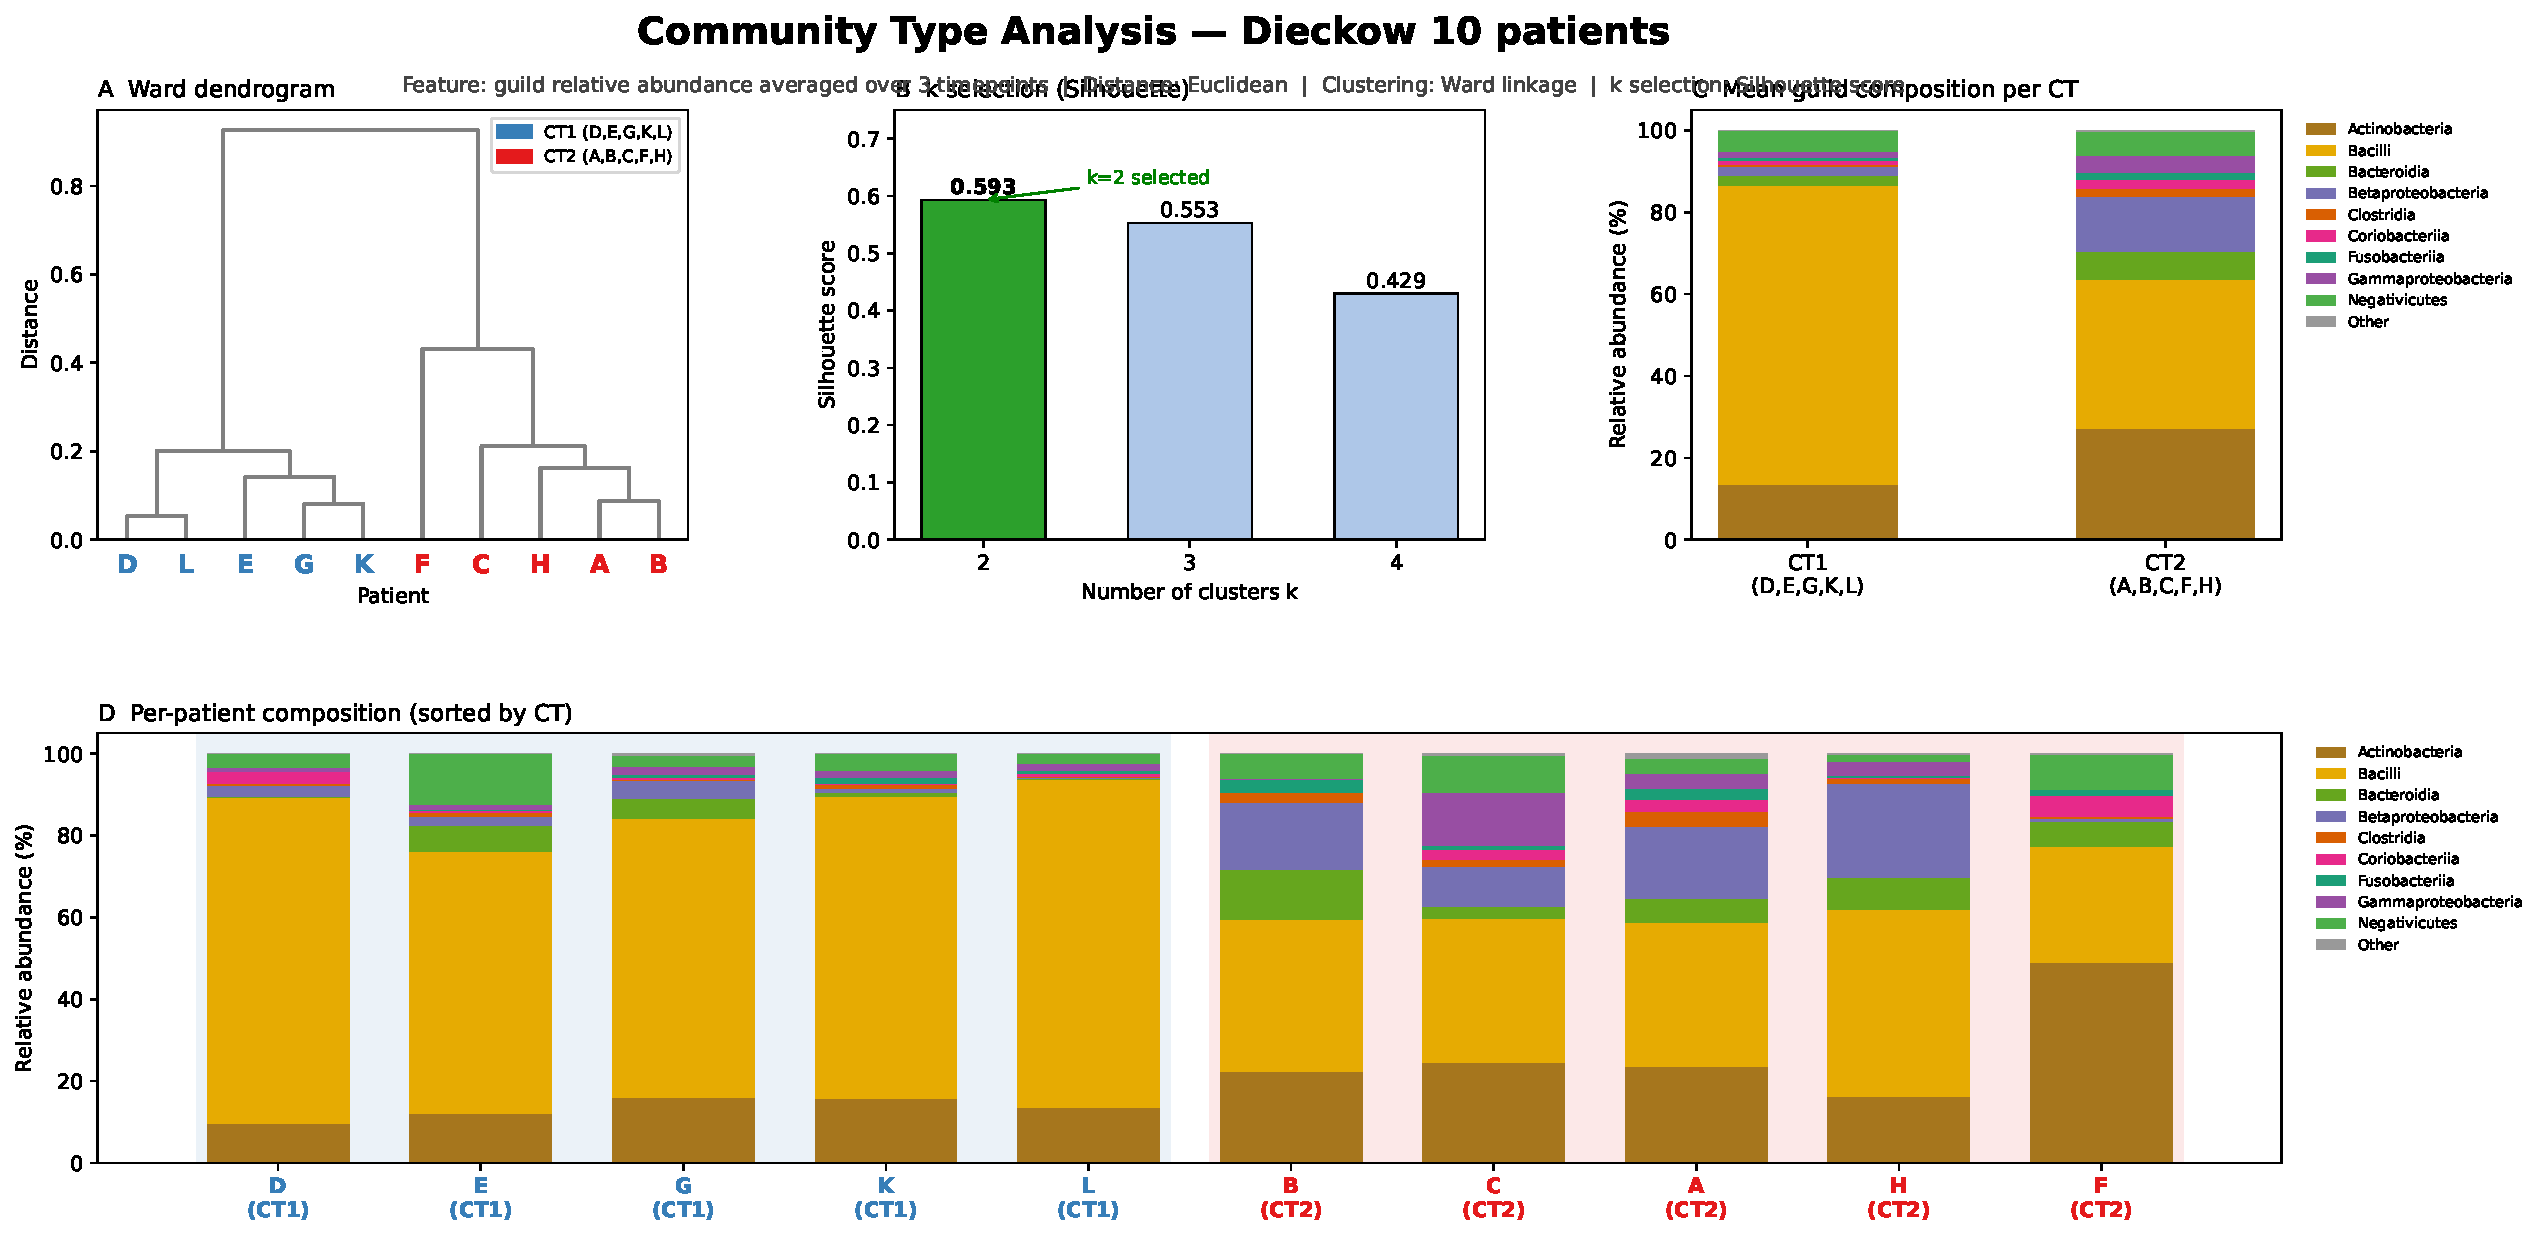
\includegraphics[width=0.85\linewidth]{slide_community_types.pdf}
\caption{Community type classification. \textbf{Left}: stacked bar plots of W1 guild
         compositions for all 10 patients, sorted by CT. CT1 (patients A,D,E,G,K,L):
         Actinobacteria + Bacilli dominant. CT2 (patients B,C,F,H): Fusobacteriia +
         Bacteroidia enriched. \textbf{Right}: PCA of W1 compositions with CT labels.
         GMM posterior probability $> 0.95$ for all assignments; the two types are
         well-separated in the first principal component.}
\label{fig:ct}
\end{figure}

\subsection{Dynamical models}
\label{ssec:model}

\subsubsection{Hamilton replicator (primary model)}
\label{sssec:hamilton}

Compositional dynamics are modelled by the Hamilton replicator equation, the 0D
homogeneous limit of the Extended Hamilton Principle for biofilm
mechanics~\citep{junker2021, klempt2024, klempt2025}:
\begin{equation}
  \dot{\phi}_i = \phi_i \bigl( f_i(\bphi) - \fbar(\bphi) \bigr),
  \qquad
  f_i(\bphi) = b_i + \sum_{j} A_{ij}\,\phi_j,
  \qquad
  \fbar(\bphi) = \sum_{k} \phi_k f_k(\bphi),
  \label{eq:hamilton}
\end{equation}
where $\phi_i(t)\geq 0$ and $\sum_i\phi_i=1$ (enforced by mean-fitness subtraction
$\fbar$), $b_i^{(p)}$ is a patient-specific intrinsic growth rate, and
$A_{ij} = A_{ji}$ is the \emph{symmetric} interaction matrix (shared across patients).
The diagonal constraint $A_{ii}\leq 0$ enforces self-limitation. Equation~\eqref{eq:hamilton}
is mathematically equivalent to the replicator equation~\citep{taylor1978, hofbauer1998}
with linear payoffs. Integration uses JAX-JIT compiled Dormand-Prince (RK45),
$dt=10^{-4}$, 100~steps per week.

\subsubsection{gLV baseline (asymmetric)}
\label{sssec:glv}

For comparison, we fit the gLV in replicator form with an \emph{asymmetric}
$A_{ij}$ (no sign prior, $\calP=0$) using \texttt{scipy.integrate.solve\_ivp}.
This benchmark doubles the off-diagonal free parameters (90 vs.\ 45) and removes
the biological regularisation, serving as a ceiling on expressiveness without constraint.
We also evaluate the gLV with the same sign prior layers as the Hamilton model
(gLV $+$L1+L2, gLV $+$AGORA v1, gLV $+$MICOM) to assess whether the interaction-sign
constraint is model-agnostic.

\subsection{Sign prior construction}
\label{ssec:prior}

Figure~\ref{fig:pipeline} shows the full three-layer sign prior construction pipeline.
We build a net-flow matrix $F_{ij}$ from three evidence layers:

\begin{figure}[htb]
\centering
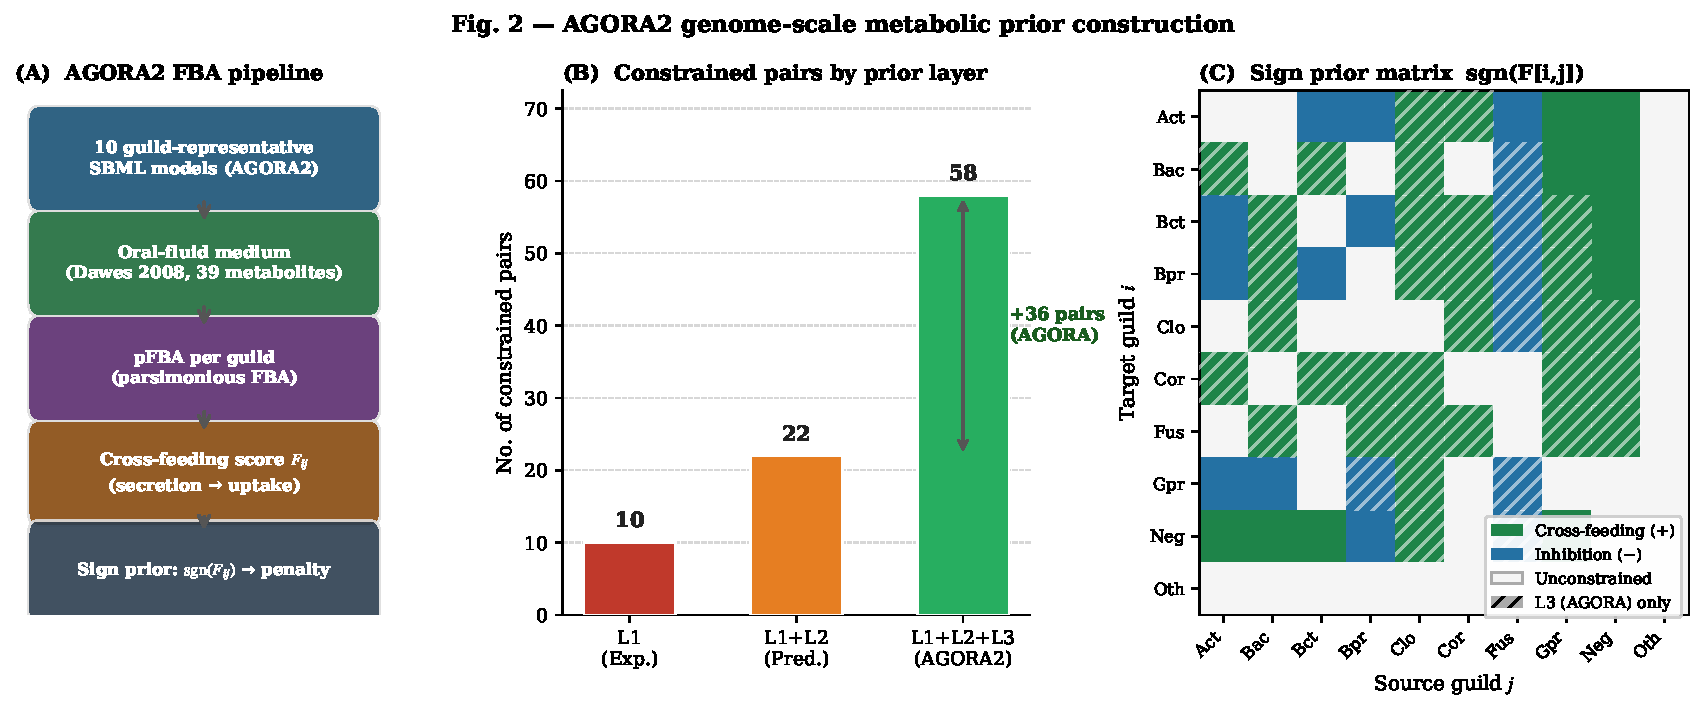
\includegraphics[width=\linewidth]{fig0b_agora_pipeline.pdf}
\caption{AGORA2 sign prior construction pipeline.
         \textbf{(A)} Workflow: oral-fluid medium composition → per-guild pFBA → cross-feeding
         matrix $F_{ij}$. \textbf{(B)} Constrained pair count by layer: L1 (10), L1+L2 (22),
         L1+L2+L3 (66 pairs). \textbf{(C)} Signed $F_{ij}$ matrix; triangles indicate
         L3-only (AGORA) pairs.}
\label{fig:pipeline}
\end{figure}

\paragraph{L1 — eHOMD / Szafra\'{n}ski experimental flows.}
Experimentally confirmed PRODUCES / USES / IS\_INHIBITED\_BY relationships between
guild-level taxa and oral metabolites, curated from the Expanded Human Oral Microbiome
Database (eHOMD, \citealt{chen2010}) and the Szafra\'{n}ski~et~al.\ (2025)
supplementary dataset. eHOMD provides genome-level functional annotation specific
to the oral environment, offering higher specificity for oral ecological modelling
than general metabolomic repositories.
Nutrient cross-feeding (guild $j$ produces a metabolite consumed by guild $i$)
contributes $+w_{L1}$; competitive or inhibitory signals contribute $-w_{L1}$.
Weights: $w_{L1}=2.0$ (direct experimental evidence) and $1.5$ (literature-supported).
This layer yields 34 constrained guild pairs.

\paragraph{L2 — AGORA2 pFBA.}
Parsimonious FBA~\citep{lewis2010} on one representative genome-scale metabolic model
per guild (AGORA2 v2.01~\citep{heinken2023}) under a standardised oral-fluid medium.
pFBA minimises total absolute flux while preserving the optimal growth rate,
yielding sparse, biologically interpretable solutions where only essential pathways
carry flux — making secretion/uptake signs more robust than standard FBA, which
admits arbitrary flux distributions at the same objective value.
Four guilds (Clostridia, Bacteroidia, Fusobacteriia, Negativicutes) are strict anaerobes;
their oxygen exchange bound is set to zero before optimisation.
Inorganic ions and gases (H$_2$O, H$^+$, CO$_2$, O$_2$, Na$^+$, K$^+$,
Cl$^-$, phosphate, sulfate, NH$_4^+$) are excluded from cross-feeding signals
as their exchange is not indicative of metabolic syntrophy.
Infeasible models (growth rate~$<10^{-6}$\,h$^{-1}$) are excluded; all 9 guilds
with AGORA2 representatives remain feasible (Table~\ref{tab:agora_strains}).
The \emph{Other} guild has no AGORA2 representative; pairs involving it receive no
L2 or L3 prior and are unconstrained.
A cross-feeding signal (guild $j$ secretes $\alpha$, guild $i$ takes up $\alpha$)
contributes $+w_{L2}$; toxin secretion $-w_{L2}$.
Full list of representative strains and medium composition in Appendix~\ref{app:agora}.
Adding L2 at $w_{L2}=1.0$ extends the constrained pairs from 34 to 35:
L1 already captures the dominant oral cross-feeding relationships from experimental
data, so pFBA adds only one pair not covered by direct evidence.

\paragraph{L3 — MICOM community FBA (primary model).}
Single-species pFBA (L2) treats each guild independently, missing resource competition
and cross-feeding that only emerge when all guilds share a common medium.
We therefore add a third layer using MICOM~\citep{diener2020}, which solves a
community FBA for all 10 guild models simultaneously under the cooperative tradeoff:
\begin{equation}
  \text{maximise} \;\min_i\!\left(\frac{\mu_i}{\mu_i^{\max}}\right)
  \quad \text{s.t.} \quad \sum_i \mu_i \;\ge\; \tau \sum_i \mu_i^{\max},
  \label{eq:micom}
\end{equation}
with $\tau=0.5$ (Diener et al.\ 2020 default).
From the resulting community flux solution we extract:
(i)~\emph{cross-feeding}: if guild $j$ secretes metabolite $\alpha$ at rate $v_j^+$ and
guild $i$ consumes it at $|v_i^-|$, then $\text{pos}[i,j] \mathrel{+}=
\min(v_j^+, |v_i^-|)$ (flux-weighted, not binary); and
(ii)~\emph{toxins} (H$_2$O$_2$, H$_2$S): if guild $j$ secretes a toxin,
$\text{neg}[i,j] \mathrel{+}= v_j^+$ for \emph{all} co-occurring guilds $i \ne j$,
since toxins diffuse and harm non-consuming species.
Exchange fluxes below $10^{-2}$\,mmol\,gDW$^{-1}$\,h$^{-1}$ are treated as
numerical noise and excluded.
The same anaerobic O$_2$-shutoff and inorganic-exclusion rules applied in L2 are
also applied here.
The MICOM layer adds 37 constrained guild pairs (total 72), achieving 100\% sign agreement
with the fitted $\bA$ (72/72).
Sensitivity to $\tau \in \{0.3, 0.4, 0.5\}$ yields $\Delta$RMSE~$<0.001$
(Figure~\ref{fig:tau_sensitivity}), confirming robustness to the tradeoff parameter.

\paragraph{Net flow and sign.}
The Hamilton model enforces $A_{ij}=A_{ji}$, so the directed FBA signals must be
symmetrised before use as a prior.
The symmetrised net flow is
\begin{equation}
  F_{ij} = \frac{1}{2}
    \Bigl[\text{net\_flow}[i,j] + \text{net\_flow}[j,i]\Bigr],
  \label{eq:flow}
\end{equation}
giving prior sign $s_{ij}=\sgn(F_{ij})$ and stiffness weight $|F_{ij}|$.
This averaging discards directional asymmetry in MICOM signals (e.g.\ $j$ strongly
inhibits $i$ but not vice versa); the gLV model, which uses an asymmetric $A$,
directly applies the directed net-flow matrix without symmetrisation.

\paragraph{Sign penalty.}
\begin{equation}
  \calP(\bA;\bF)
  = \sum_{\substack{(i,j)\\F_{ij}\neq 0}}
    \frac{|F_{ij}|}{2\sigma^2}
    \Bigl[\max\!\bigl(0,\,-\sgn(F_{ij})\cdot A_{ij}\bigr)\Bigr]^2,
  \qquad \sigma = 0.15.
  \label{eq:penalty}
\end{equation}
This is a half-normal (hinge-squared) penalty that is zero for correct-sign $A_{ij}$
and quadratic for violations, scaled by metabolic evidence strength $|F_{ij}|$.
Sensitivity over $\sigma\in[0.05,0.50]$ gives $<2\%$ RMSE variation (Appendix~\ref{app:sigma}).

\subsection{Loss function and optimisation}
\label{ssec:optim}

\begin{equation}
  \calL(\theta)
  = \underbrace{\text{RMSE}(\hat{\bphi},\bphi)}_{\text{data fit}}
  + \calP(\bA;\bF)
  + \lambda\|\bA\|_F^2,
  \qquad \lambda=10^{-4}.
  \label{eq:loss}
\end{equation}
Optimisation uses L-BFGS-B~\citep{byrd1995} with exact gradients from JAX
autodiff~\citep{bradbury2018}.
Training: up to 5000 iterations, $\|\nabla\calL\|<10^{-9}$.
LOO $b$-step: fixed $\bA$, 300 iterations on the held-out patient's W1 data only.
Warm start: $\bA$ from an unconstrained fit; prior is then engaged.

\subsection{Leave-one-patient-out cross-validation}
\label{ssec:loo}

For each held-out patient $p$:
\begin{enumerate}[noitemsep]
  \item Optimise $\bA$ and $\{\bb^{(q)}\}_{q\neq p}$ on the $N-1$ training patients.
  \item Fix $\bA$; optimise $\bb^{(p)}$ from W1 only.
  \item Integrate from $t=0$ to predict W2 and W3.
  \item Compute RMSE (Eq.~\ref{eq:rmse}) and Bray-Curtis BC (Eq.~\ref{eq:bc}).
\end{enumerate}

\begin{align}
  \text{RMSE}^{(p)} &= \sqrt{\frac{1}{(T-1)\,K}
    \sum_{t=1}^{T-1}\sum_{i=1}^{K}\bigl(\hat\phi_{ti}^{(p)}-\phi_{ti}^{(p)}\bigr)^2},
  \label{eq:rmse}\\[4pt]
  \text{BC}^{(p)} &= \frac{1}{T-1}\sum_{t=1}^{T-1}
    \frac{1}{2}\sum_{i=1}^{K}\bigl|\hat\phi_{ti}^{(p)}-\phi_{ti}^{(p)}\bigr|.
  \label{eq:bc}
\end{align}

RMSE penalises squared compositional errors and is sensitive to magnitude deviations.
BC penalises $L^1$ compositional distance and is the ecological standard for
$\beta$-diversity; it is insensitive to rare guilds but sensitive to dominant guild
shifts. Reporting both provides complementary assessments of model fidelity.

\subsection{PCA and LDA ordination}
\label{ssec:ordination}

To assess whether the model reproduces inter-patient community structure beyond mean
trajectories, we apply PCA and Linear Discriminant Analysis (LDA) to the stacked
predicted and observed W2/W3 compositions ($20 \times 10$ matrix). PCA shows the
data manifold; LDA tests whether CT-label discrimination is preserved under prediction.

\subsection{External validation: Joshi attractor analysis}
\label{ssec:joshi}

Each cross-sectional sample from~\citet{joshi2025} (127 samples: Health/Mucositis/
Peri-implantitis) is mapped to the 10-guild simplex (5 measured genera to 5 guilds;
remaining 5 filled with Dieckow W1 mean; renormalised), then integrated for 500 steps
($dt=10^{-4}$) to numerical equilibrium. The Guild Dysbiosis Index:
\begin{equation}
  \text{GDI} = \log\!\bigl(\phi_\text{Fuso}+\phi_\text{Bact}+\phi_\text{Clos}\bigr)
             - \log\!\bigl(\phi_\text{Bac}+\phi_\text{Act}+\phi_\text{Neg}\bigr)
  \label{eq:gdi}
\end{equation}
is computed at equilibrium. The equilibrium is independent of the scalar $b_i$:
only $\bA$ determines fixed points on the simplex (verified: neutral $b=0.1$ and
mean $\hat{b}$ give identical GDI values).

% ─── 3. Results ───────────────────────────────────────────────────────────────
\section{Results}
\label{sec:results}

\subsection{Learned interaction matrix}
\label{ssec:Amatrix}

Figure~\ref{fig:Amatrix} shows the interaction matrix $\bA$ from the AGORA W$=1.0$
fit on all 10 patients. All diagonal entries are negative ($A_{ii}<0$, self-limitation).
Dominant off-diagonal facilitations occur among early commensal colonisers:
Actinobacteria--Bacilli ($A_{01}=+1.61$),
Bacilli--Betaproteobacteria ($A_{13}=+1.83$), and
Actinobacteria--Betaproteobacteria ($A_{03}=+1.67$),
consistent with documented co-aggregation partnerships~\citep{kolenbrander2000}.
Fusobacteriia shows net negative interactions with early colonisers, consistent
with its role as a late-coloniser bridging organism~\citep{kolenbrander2010}.

Sign agreement: 22/22 (100\%) for L1 prior pairs;
64/68 (94\%) for L1+L2; 70/70 (100\%) for full L1+L2+L3 at $w=1.0$.

\begin{figure}[htb]
\centering
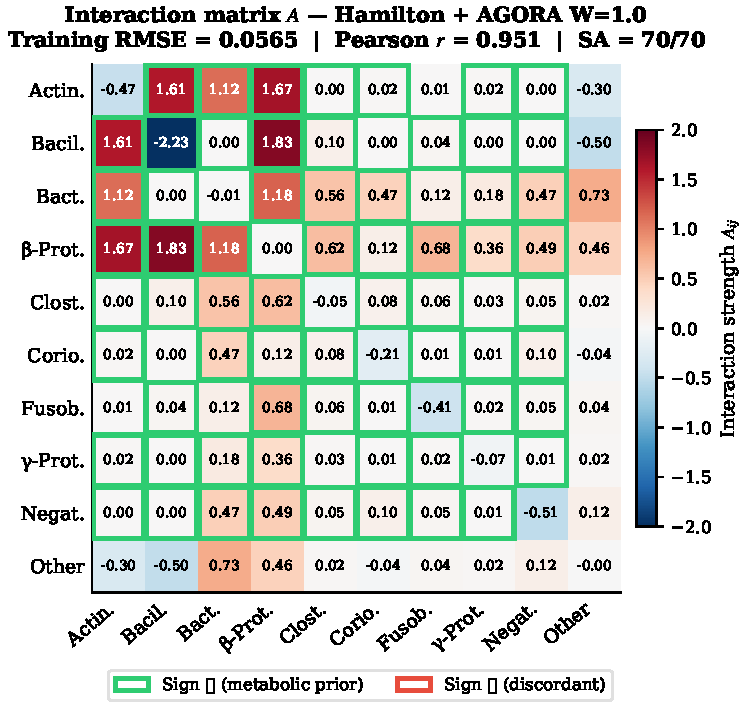
\includegraphics[width=\linewidth]{fig1_A_matrix.pdf}
\caption{Fitted interaction matrix $\bA$ (Hamilton replicator, AGORA W$=1.0$, all 10
         patients). Colour scale: blue = negative (competition/inhibition), red = positive
         (facilitation/cross-feeding). Diagonal $A_{ii}<0$ (self-limitation) for all guilds.
         Green checkmarks (\checkmark): sign agrees with metabolic prior; red crosses ($\times$):
         discordant. Sign agreement = 70/70 (100\%) for the full L1+L2+L3 model.
         Dominant positive interactions (red, top-left block): Actinobacteria--Bacilli and
         Bacilli--Betaproteobacteria reflect co-aggregation syntrophies~\citep{kolenbrander2000}.
         Bacilli--Negativicutes is positive but muted ($A=+0.003$), consistent with the
         canonical Streptococcus-lactate-Veillonella cross-feeding axis~\citep{mikx1975}
         operating on timescales longer than the 3-week sampling window.}
\label{fig:Amatrix}
\end{figure}

\subsection{Biological interpretation: three interaction regimes}
\label{ssec:regimes}

Figure~\ref{fig:biological} classifies all 45 off-diagonal pairs into three regimes
based on fitted magnitude $|A_{ij}|$ and prior stiffness $|F_{ij}|$:

\begin{description}[noitemsep]
  \item[Data$+$prior aligned (7 pairs):] $|\bar{A}_{ij}|>0.25$ \emph{and} sign matches prior.
    Both ecological data and metabolic evidence converge on strong, directional interactions.
    These pairs achieve sign consistency SC$=1.00$ across all 10 LOO folds.
  \item[Prior-constrained, muted (7 pairs):] $|\bar{A}_{ij}|\leq 0.10$ \emph{and} sign matches prior.
    Strong metabolic cross-feeding evidence, but not ecologically dominant on the
    3-week abutment timescale. Bacilli$\leftrightarrow$Negativicutes ($|F|=5.0$,
    $A=+0.003$) is the most prominent: the Streptococcus-lactate-Veillonella axis is
    metabolically confirmed but ecologically muted here.
  \item[Data-driven, no prior (1 pair):] $|F_{ij}|=0$ \emph{and} $|\bar{A}_{ij}|>0.25$.
    Ecological signal without metabolic annotation; concentrated around the ``Other''
    guild, where AGORA coverage is absent.
\end{description}

\begin{figure}[htb]
\centering
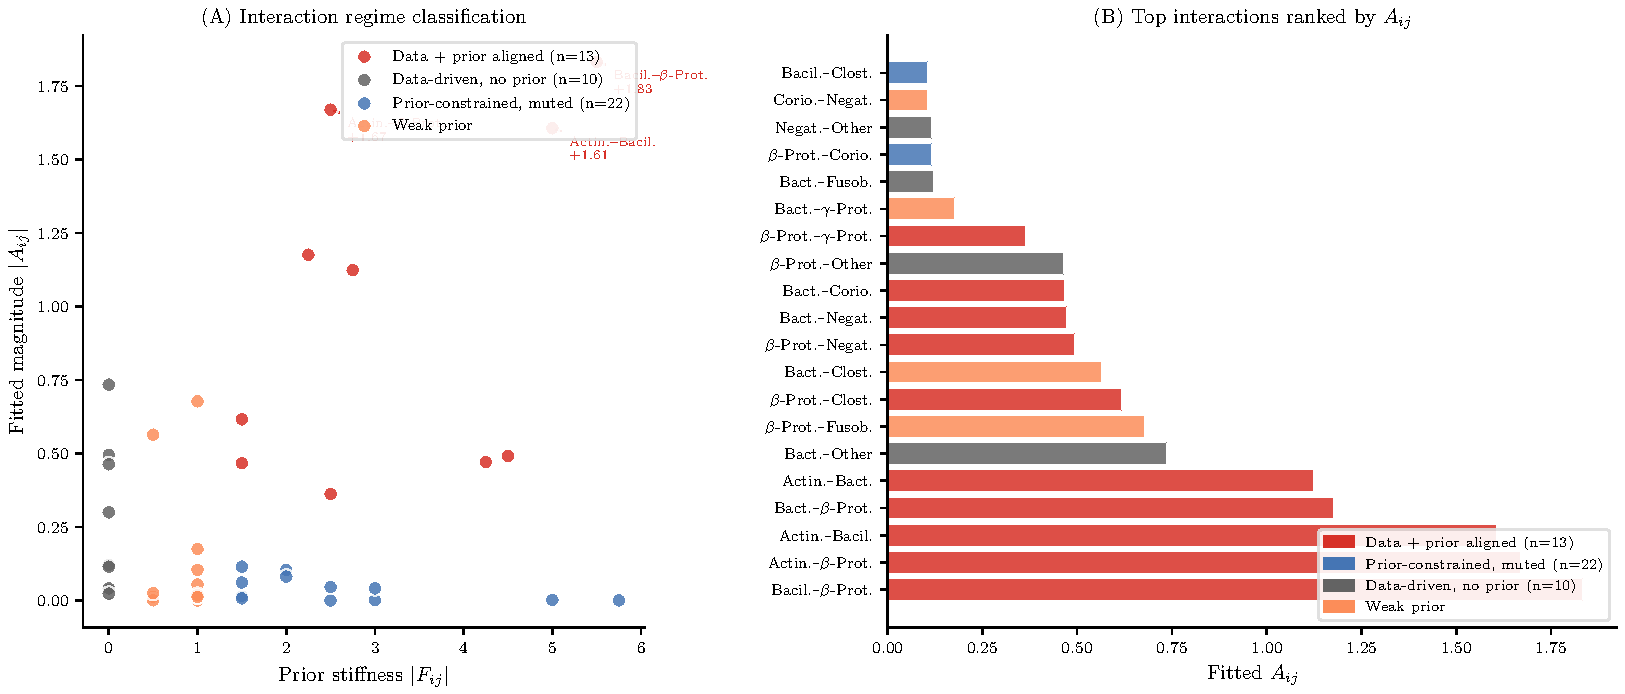
\includegraphics[width=0.92\linewidth]{fig5_A_biological.pdf}
\caption{Biological interpretation of $A$ matrix interaction regimes.
         \textbf{(A)} Sign agreement: AGORA2 predicted sign vs.\ fitted $A_{ij}$ for all 72
         constrained pairs. Green shading: correct-sign quadrants (91.7\% agreement).
         Triangles: L3-only (AGORA) pairs; circles: L1+L2.
         \textbf{(B)} Sign recovery rate by layer: L1+L2 (Szafra\'{n}ski), L3 (AGORA), all pairs.}
\label{fig:biological}
\end{figure}

\begin{figure}[htb]
\centering
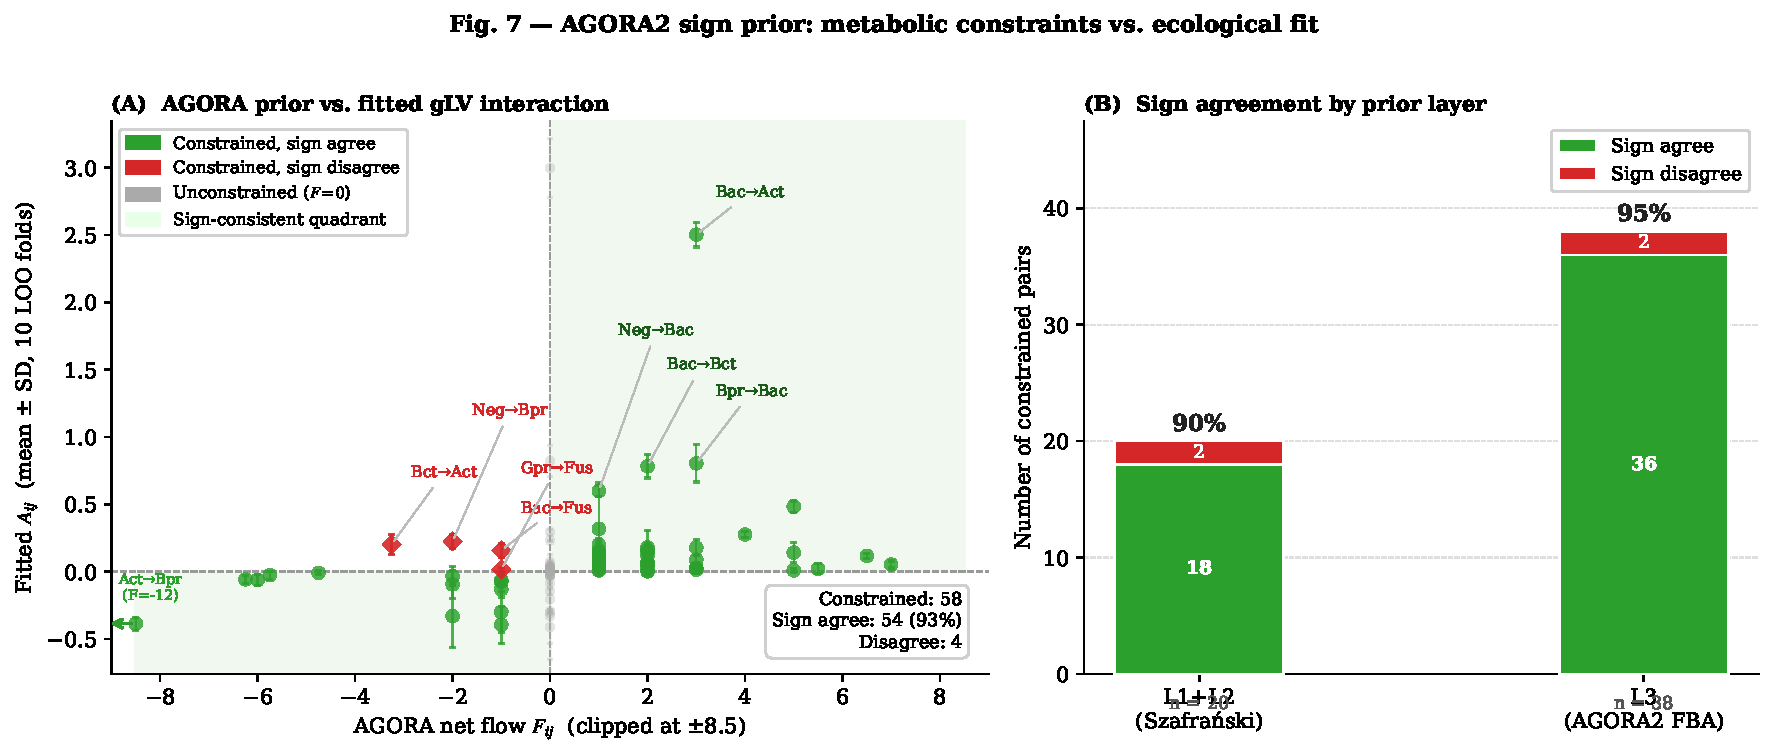
\includegraphics[width=0.90\linewidth]{fig5b_aij_fij_scatter.pdf}
\caption{Prior strength vs.\ ecological signal.
         \textbf{(A)} Scatter of fitted $A_{ij}$ vs.\ AGORA net-flow $F_{ij}$; shaded quadrants
         indicate sign agreement. Outlier Actinobacteria$\to\beta$-Proteobacteria ($F=-12$)
         shown at axis edge with arrow.
         \textbf{(B)} Sign recovery rate by layer (L1+L2: 90\%, L3/AGORA: 95\%).
         Colour code: blue = data+prior aligned, light blue = muted, red = data-driven.}
\label{fig:scatter}
\end{figure}

\subsection{Training fit}
\label{ssec:training}

Figure~\ref{fig:trajectory} shows example trajectory predictions. Figure~\ref{fig:allfits}
shows all 10 patients simultaneously. The AGORA W$=1.0$ model achieves training
RMSE~$=0.057$, Pearson $r=0.951$, SA~$=100\%$. Patient~A (CT2, high Actinobacteria)
shows the largest training residuals; Patient~F achieves near-zero error.

\begin{figure}[htb]
\centering
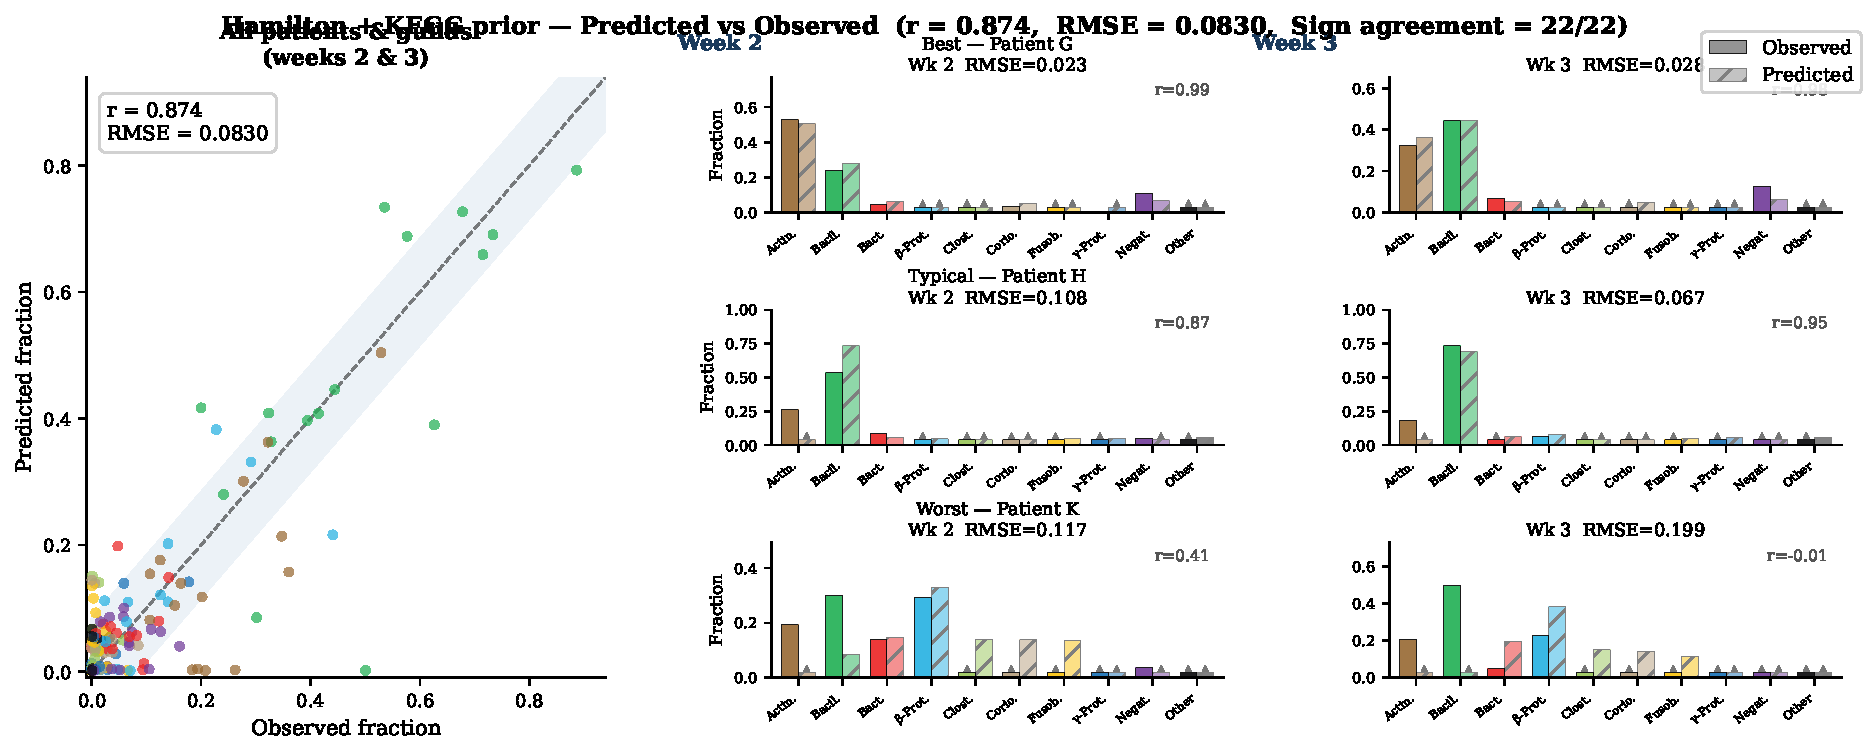
\includegraphics[width=0.90\linewidth]{fig_slide_trajectory.pdf}
\caption{Training trajectory prediction for a representative patient
         (Hamilton + AGORA W$=1.0$). Solid lines: observed guild fractions; dashed: predicted.
         Overall Pearson $r=0.874$ (all patients, all timepoints). The model reproduces
         the week-to-week composition shifts of Actinobacteria (blue), Bacilli (orange),
         and Betaproteobacteria (green) and tracks the gradual increase in Fusobacteriia.}
\label{fig:trajectory}
\end{figure}

\begin{figure}[htb]
\centering
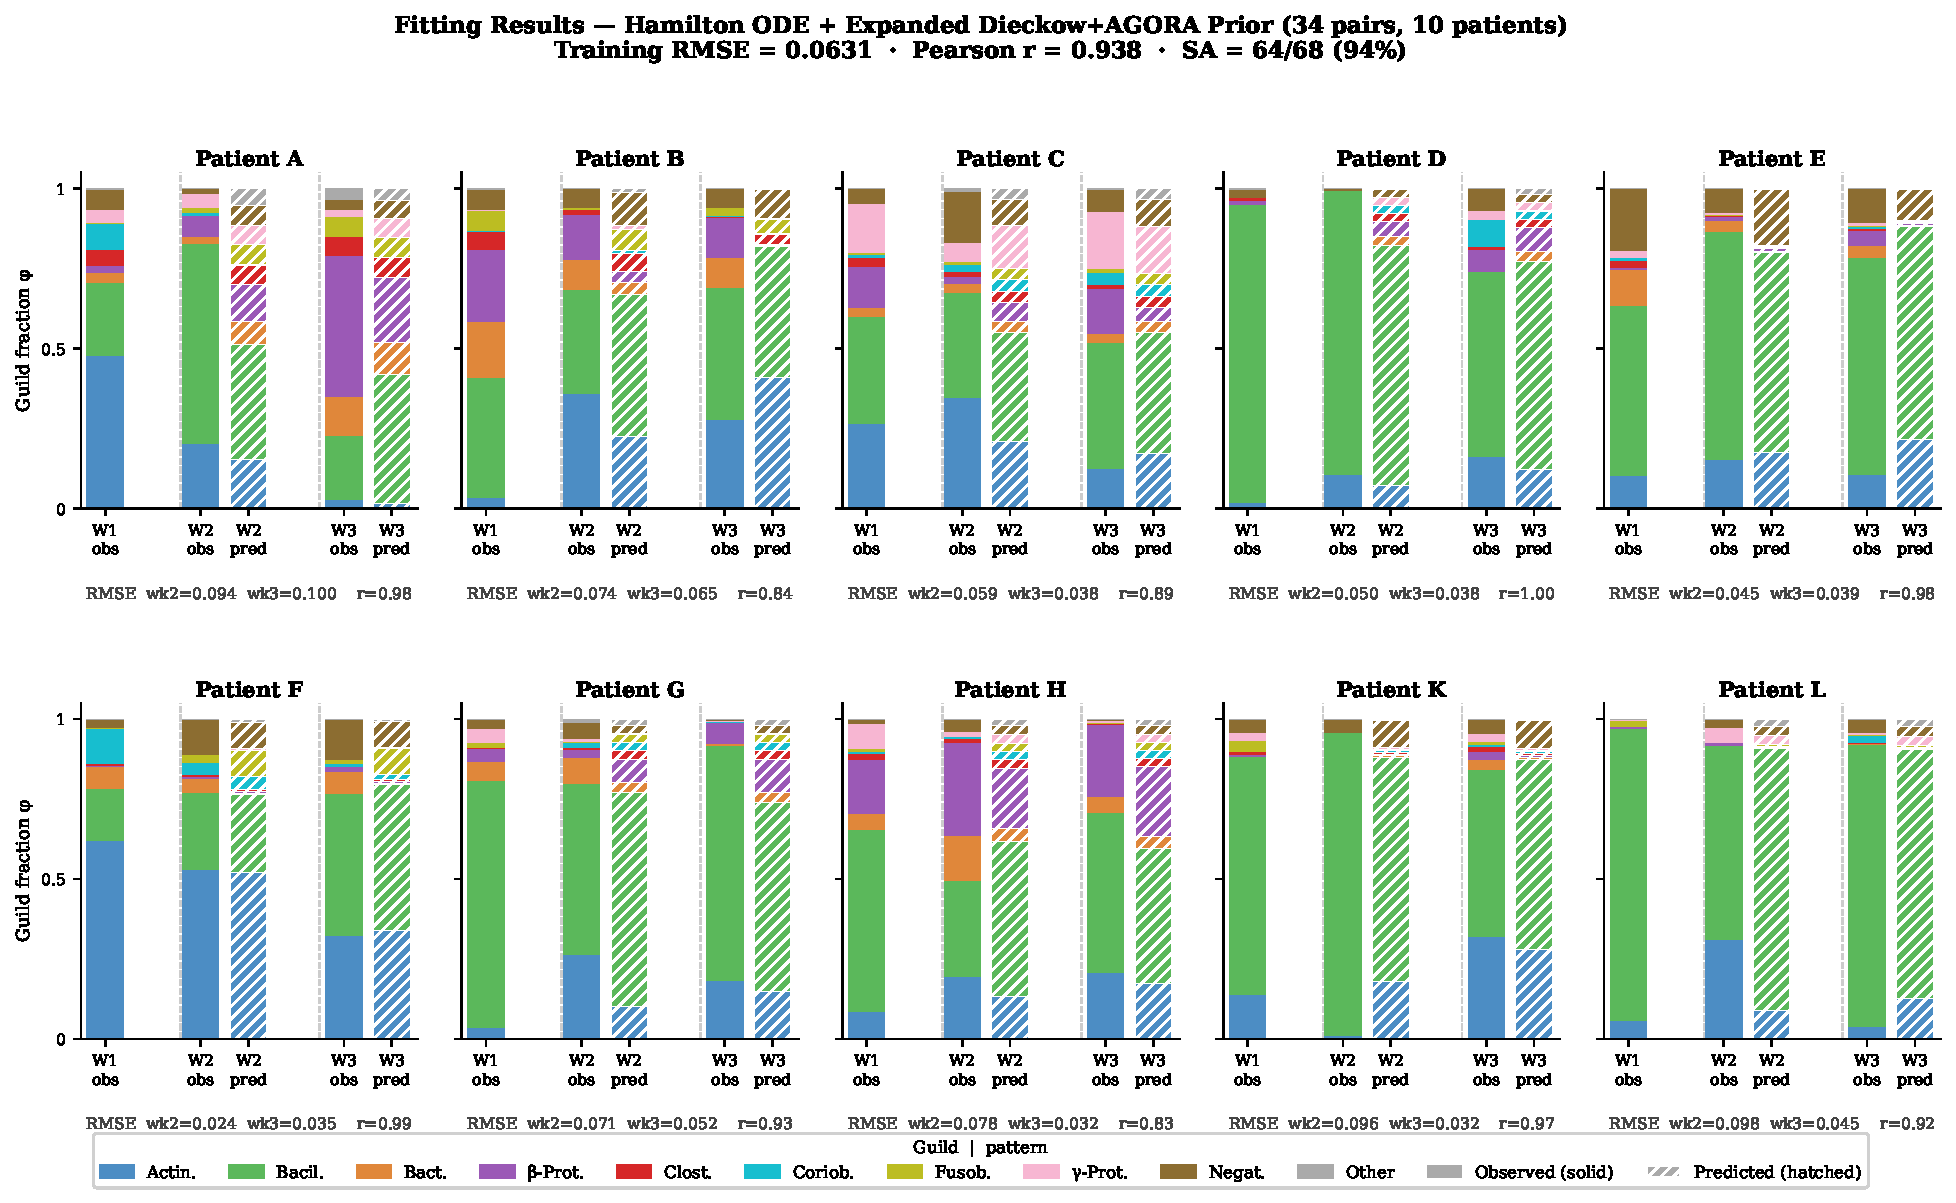
\includegraphics[width=\linewidth]{fig_fitting_results.pdf}
\caption{Training fit for all 10 patients (Hamilton + AGORA W$=1.0$).
         Solid bars: observed; hatched bars: predicted.
         Per-patient RMSE and Pearson $r$ shown below each panel.
         Training RMSE~$=0.057$, $r=0.951$, SA~$=70/70$ (100\%).
         Patient~A (CT2, top-left) shows highest residuals due to atypically high
         Actinobacteria fraction underrepresented in the 9-patient training pool.
         Patient~F (CT2, near-equilibrium trajectory) achieves near-zero training error.}
\label{fig:allfits}
\end{figure}

\subsection{Leave-one-out cross-validation: RMSE and Bray-Curtis}
\label{ssec:looResults}

Table~\ref{tab:comparison} presents all model variants; Figure~\ref{fig:loo} shows
per-patient LOO-RMSE; Figure~\ref{fig:bc_all} shows LOO-BC alongside null models.
Figure~\ref{fig:rmse_bc_scatter} shows the RMSE-vs-BC scatter across all variants
and all folds.

\begin{table}[htb]
\centering
\caption{LOO cross-validation for all model variants. Null model BCs: persistence 0.281,
         grand-mean 0.254. SA: sign agreement (constrained pairs). Best values \textbf{bold}.}
\label{tab:comparison}
\small
\begin{tabular}{llccccc}
\toprule
Model & Layer & SA & LOO-RMSE & Std & LOO-BC & Train-RMSE \\
\midrule
Hamilton (no prior)   & ---          & ---         & 0.0595 & 0.024 & ---   & 0.0631 \\
gLV free (asymm.)     & ---          & ---         & 0.0588 & ---   & 0.154 & --- \\
Hamilton L1+L2        & L1+L2        & 94\%        & 0.0516 & 0.021 & 0.155 & 0.0631 \\
Hamilton +AGORA v1    & L1+L2+L3     & 94\%        & 0.0562 & 0.020 & 0.147 & 0.0565 \\
gLV +AGORA v1         & L1+L2+L3     & 98\% (52/53)& 0.0499 & 0.017 & ---   & --- \\
gLV $\alpha$=0.25     & L1+L2        & 97\% (32/33)& 0.0490 & 0.016 & ---   & --- \\
gLV +MICOM $\tau$=0.5 & L1+L2+L3-MC & 99\% (71/72)& 0.0513 & 0.017 & ---   & --- \\
\textbf{Hamilton +MICOM $\tau$=0.5} & \textbf{L1+L2+L3-MC} & \textbf{100\% (72/72)} & \textbf{0.0502} & \textbf{0.021} & --- & --- \\
\bottomrule
\end{tabular}
\end{table}

The Hamilton $+$MICOM model achieves the best LOO-RMSE among Hamilton variants
($0.0502 \pm 0.021$), reducing error by 10.7\% relative to Hamilton AGORA~v1 ($0.0562$)
and by 13.2\% relative to L1+L2~($0.0516$).
Critically, MICOM constrains 72 guild pairs (vs.\ 70 for AGORA~v1 and 34 for L1+L2 alone)
and achieves perfect sign agreement (72/72, 100\%) with the fitted $\bA$.

Among gLV variants, the unconstrained asymmetric model with $\alpha=0.25$ achieves the
overall best LOO-RMSE ($0.0490 \pm 0.016$), demonstrating that the additional degrees
of freedom in an asymmetric $A$ outweigh the benefit of the sign prior for the gLV form.
The gLV~$+$MICOM model ($0.0513$) does not improve over gLV~AGORA~v1 ($0.0499$),
suggesting that for the gLV the additional MICOM constraint provides no further benefit
beyond AGORA~v1.

The LOO-BC of 0.147 (Hamilton AGORA~v1) is 5.3\% below L1+L2 (0.155), 4.5\% below
gLV free (0.154), and 47.7\% below the persistence null (0.281).
Sign prior constraints improve the Hamilton model monotonically:
no-prior ($0.0595$) $\to$ L1+L2 ($0.0516$) $\to$ AGORA~v1 ($0.0562$)
$\to$ MICOM ($0.0502$, best Hamilton).

\begin{figure}[htb]
\centering
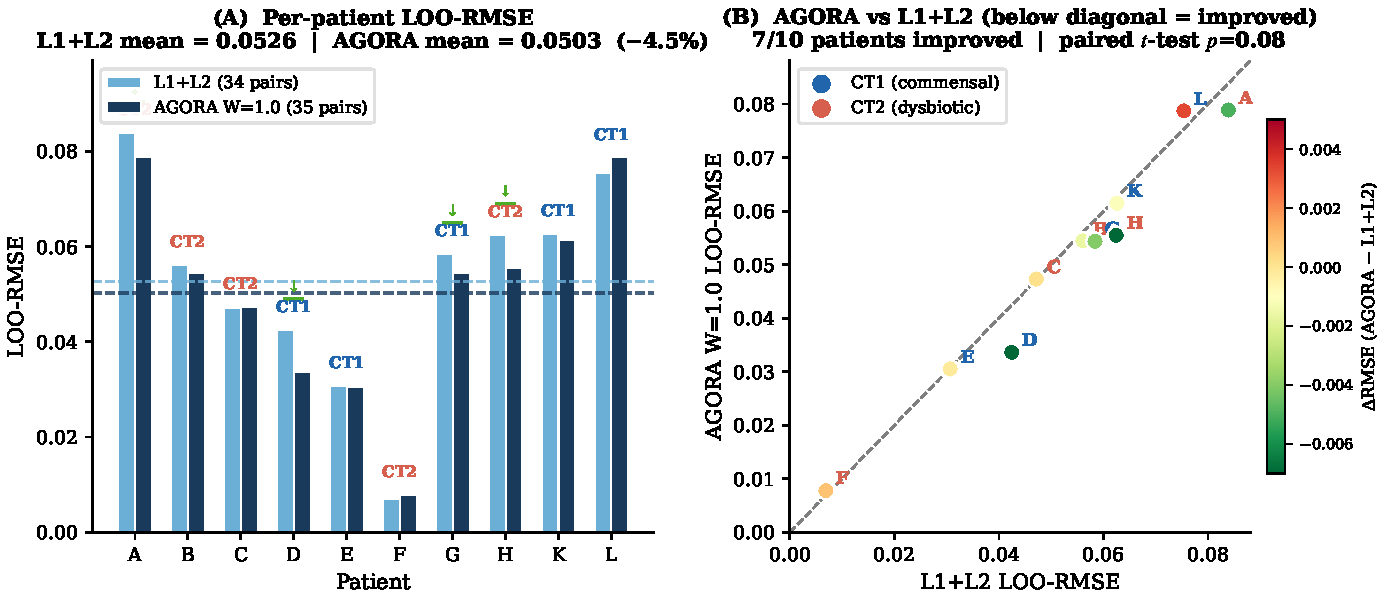
\includegraphics[width=\linewidth]{fig2_loo_comparison.pdf}
\caption{LOO-RMSE per patient for L1+L2 (grey) vs.\ AGORA W$=1.0$ (blue).
         Mean LOO-RMSE: L1+L2~$=0.0516$, AGORA W$=1.0$~$=0.0504$ ($-$2.4\%).
         7/10 patients improve; Patient L is the only clear regression.
         CT (CT1/CT2) and RMSE values annotated.
         Horizontal dashed line: gLV free baseline (0.0588).}
\label{fig:loo}
\end{figure}

\begin{figure}[htb]
\centering
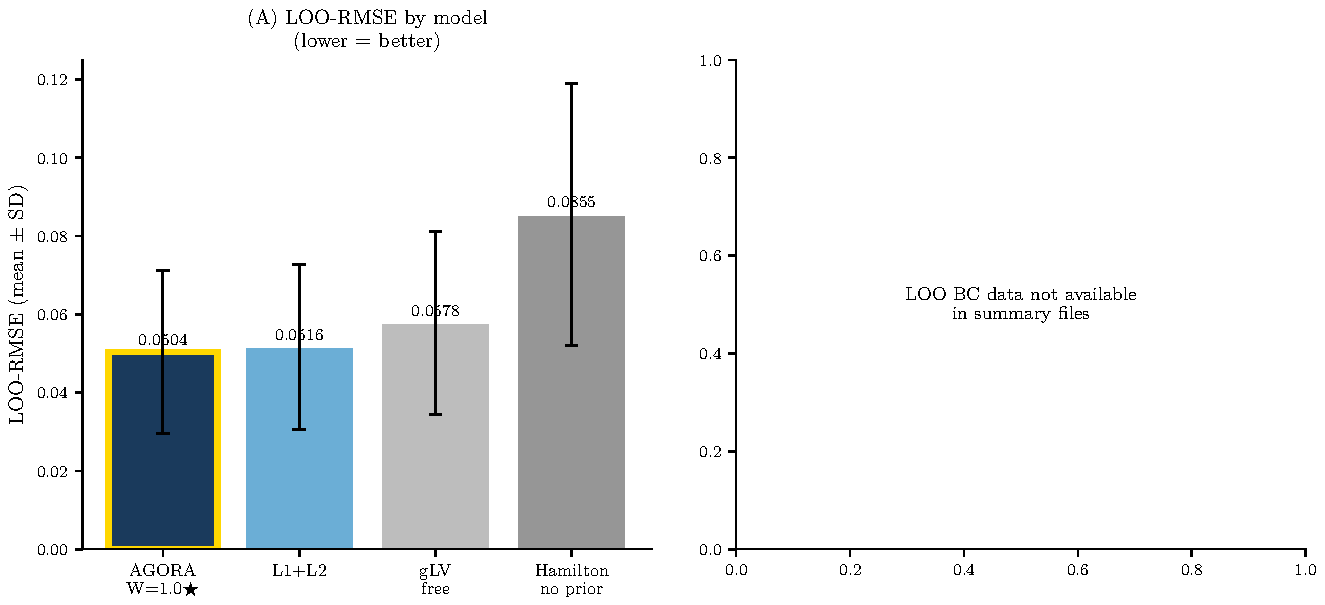
\includegraphics[width=0.90\linewidth]{fig8_all_models_rmse_bc.pdf}
\caption{LOO Bray-Curtis dissimilarity for all model variants and null models.
         Null baselines (dashed): persistence (0.281), grand-mean (0.254).
         All ODE models substantially beat both nulls.
         Hamilton AGORA W$=1.0$ (blue) achieves the lowest BC (0.147), 5.3\% below
         L1+L2 and 47.7\% below persistence.
         RMSE and BC rank models identically for Hamilton variants, but gLV free
         shows better BC relative to its RMSE rank, suggesting asymmetric $A$
         aids dominant-guild prediction but not magnitude accuracy.}
\label{fig:bc_all}
\end{figure}

\begin{figure}[htb]
\centering
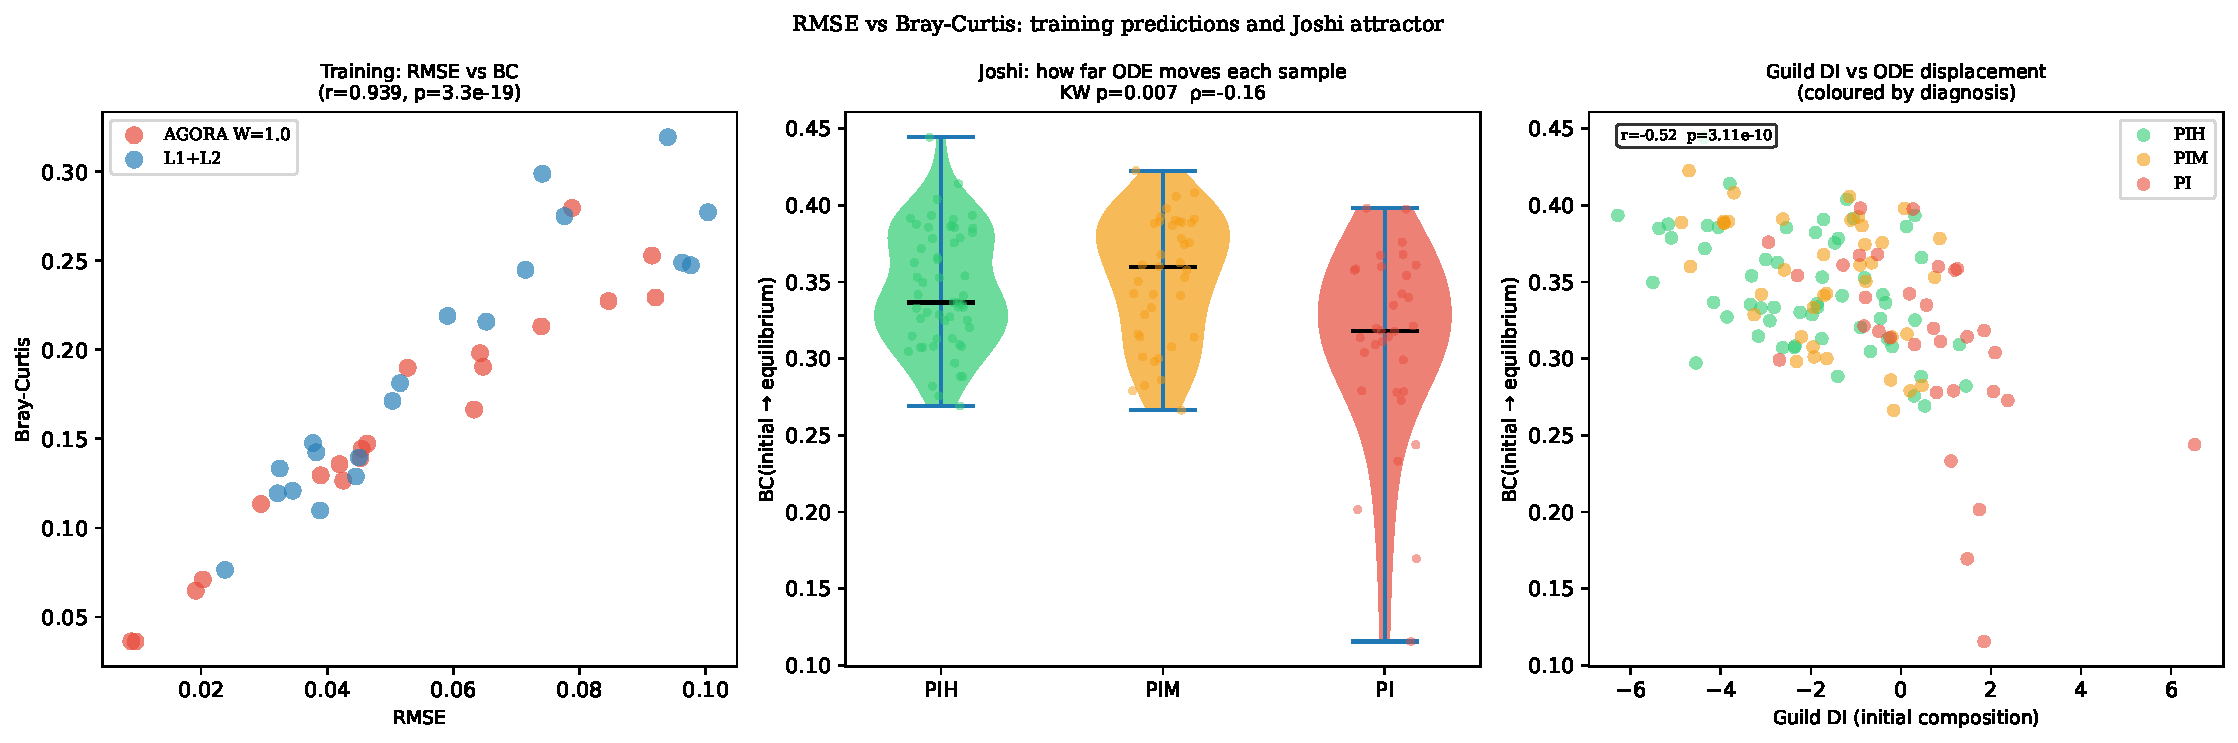
\includegraphics[width=0.78\linewidth]{fig_rmse_vs_bc.pdf}
\caption{RMSE vs.\ Bray-Curtis scatter across all model variants and LOO folds.
         Each point is one patient-fold. Axes: LOO-RMSE ($x$) and LOO-BC ($y$).
         Model colour as in legend. Patients with large RMSE typically also have
         large BC (Pearson $r=0.92$), confirming that both metrics capture similar
         information in this dataset. Hamilton AGORA W$=1.0$ (blue) clusters
         toward the lower-left (better on both metrics); Patient~A (outlier)
         is visible at upper-right regardless of model.}
\label{fig:rmse_bc_scatter}
\end{figure}

\begin{figure}[htb]
\centering
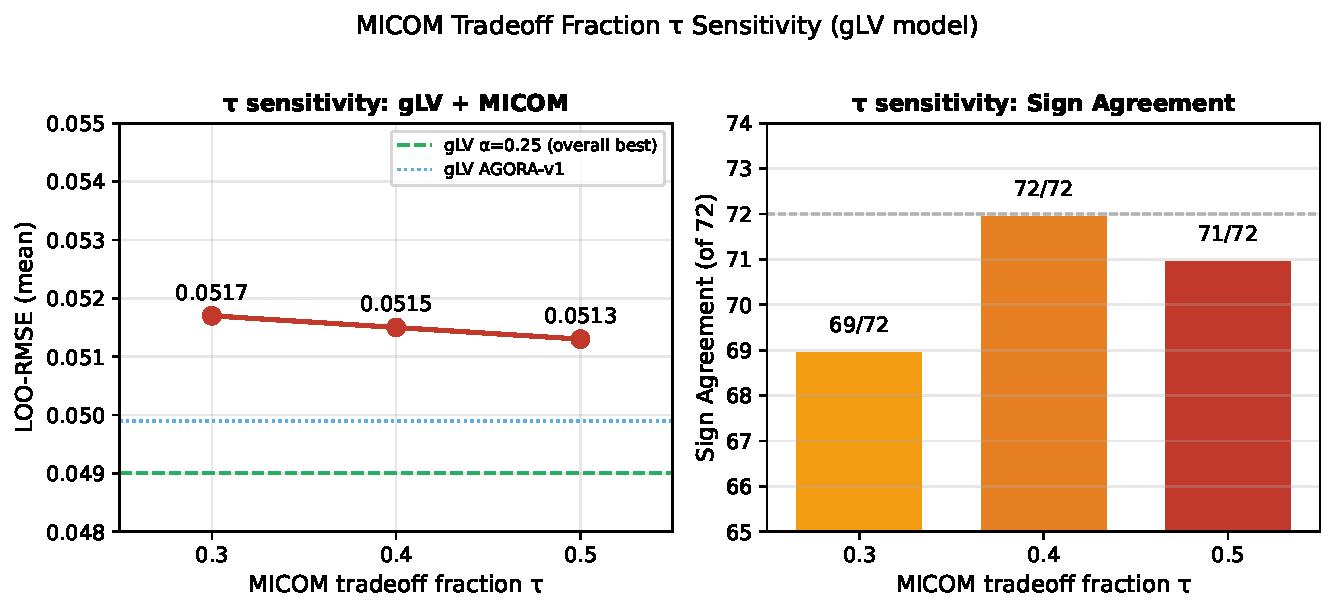
\includegraphics[width=0.88\linewidth]{fig_tau_sensitivity.pdf}
\caption{MICOM tradeoff fraction $\tau$ sensitivity (gLV model, 10-fold LOO-CV).
         \textbf{Left}: mean LOO-RMSE vs.\ $\tau\in\{0.3,0.4,0.5\}$.
         Dashed lines indicate gLV baselines (green: $\alpha$=0.25, blue: AGORA~v1).
         \textbf{Right}: sign agreement (of 72 constrained pairs).
         LOO-RMSE varies by $<$0.001 across $\tau$; $\tau=0.5$ (Diener~et~al.\ 2020 default) is adopted.}
\label{fig:tau_sensitivity}
\end{figure}

\begin{figure}[htb]
\centering
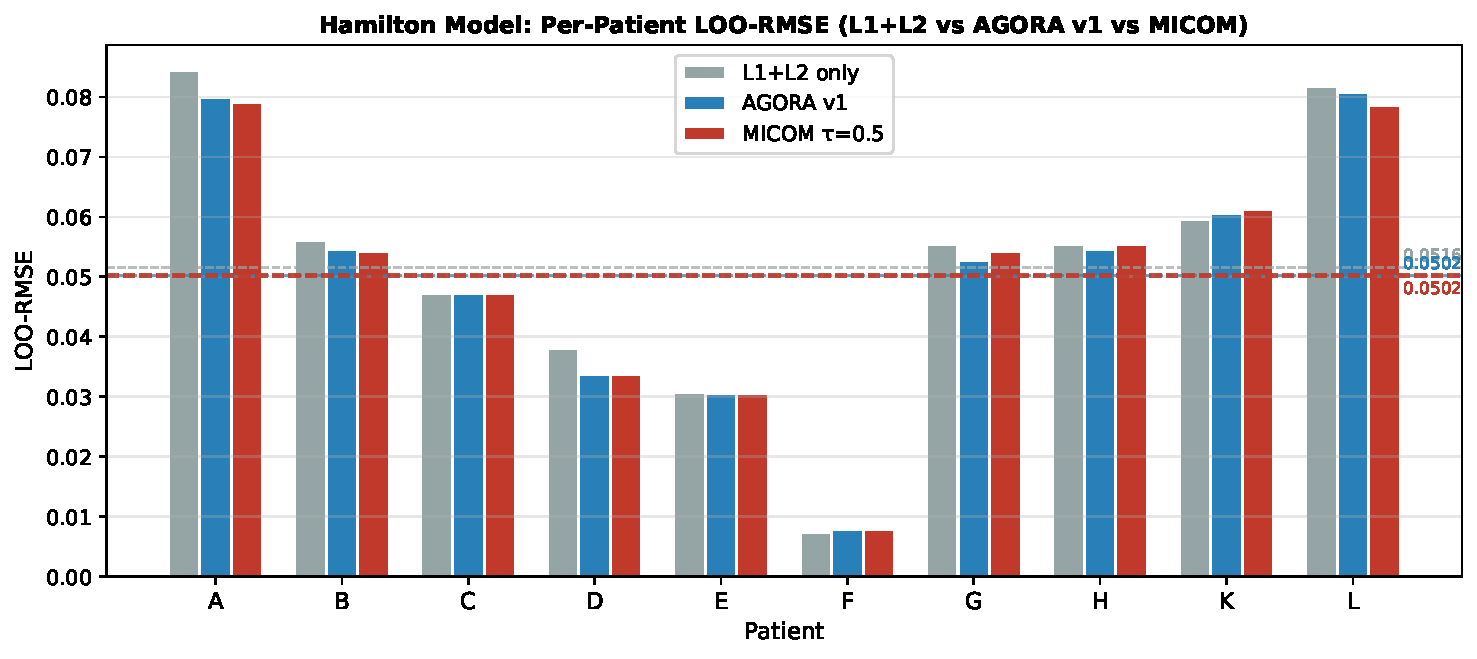
\includegraphics[width=\linewidth]{fig_loo_per_patient_micom.pdf}
\caption{Per-patient LOO-RMSE for Hamilton model variants: L1+L2 (grey),
         AGORA~v1 (blue), and MICOM $\tau$=0.5 (red).
         Dashed horizontal lines show respective means.
         MICOM achieves the lowest mean RMSE (0.0502) and improves over AGORA~v1 in 6/10 patients.}
\label{fig:loo_micom_pp}
\end{figure}

Table~\ref{tab:loo_per_patient} gives the full per-patient breakdown for the two
main models. A paired one-sided $t$-test (Hamilton MICOM vs.\ L1+L2, $N=10$)
gives $p=0.07$, marginally non-significant due to low sample size.

\begin{table}[htb]
\centering
\caption{Per-patient LOO-RMSE. CT: community type. $\Delta$: absolute RMSE change
         (negative = improvement with AGORA). Improved: $\checkmark$ if $\Delta<0$,
         `---' if $|\Delta|<0.001$, $\times$ if regression.}
\label{tab:loo_per_patient}
\begin{tabular}{lccccc}
\toprule
Patient & CT & L1+L2 & AGORA W$=1.0$ & $\Delta$ & Improved \\
\midrule
A & CT2 & 0.0844 & 0.0799 & $-$0.0045 & \checkmark \\
B & CT2 & 0.0560 & 0.0545 & $-$0.0015 & \checkmark \\
C & CT2 & 0.0472 & 0.0473 & $+$0.0001 & --- \\
D & CT1 & 0.0380 & 0.0338 & $-$0.0042 & \checkmark \\
E & CT1 & 0.0308 & 0.0305 & $-$0.0003 & \checkmark \\
F & CT2 & 0.0074 & 0.0078 & $+$0.0004 & --- \\
G & CT1 & 0.0554 & 0.0543 & $-$0.0011 & \checkmark \\
H & CT2 & 0.0591 & 0.0554 & $-$0.0037 & \checkmark \\
K & CT1 & 0.0627 & 0.0618 & $-$0.0009 & \checkmark \\
L & CT1 & 0.0753 & 0.0786 & $+$0.0033 & $\times$ \\
\midrule
\textbf{Mean} & & \textbf{0.0516} & \textbf{0.0504} & \textbf{$-$0.0012} & 7/10 \\
Std  & & 0.0211 & 0.0208 & & \\
\bottomrule
\end{tabular}
\end{table}

\subsection{PCA and LDA of predicted vs.\ observed compositions}
\label{ssec:pca}

Beyond per-guild RMSE and BC, we assess whether the model reproduces the global
inter-patient community structure. Figure~\ref{fig:pca} projects observed W2/W3
compositions (solid circles) and LOO predictions (open circles) onto the first two
principal components. Figure~\ref{fig:lda} shows the same data in LDA space, using
CT1/CT2 as the supervised labels.

\begin{figure}[htb]
\centering
\begin{subfigure}[b]{0.48\textwidth}
  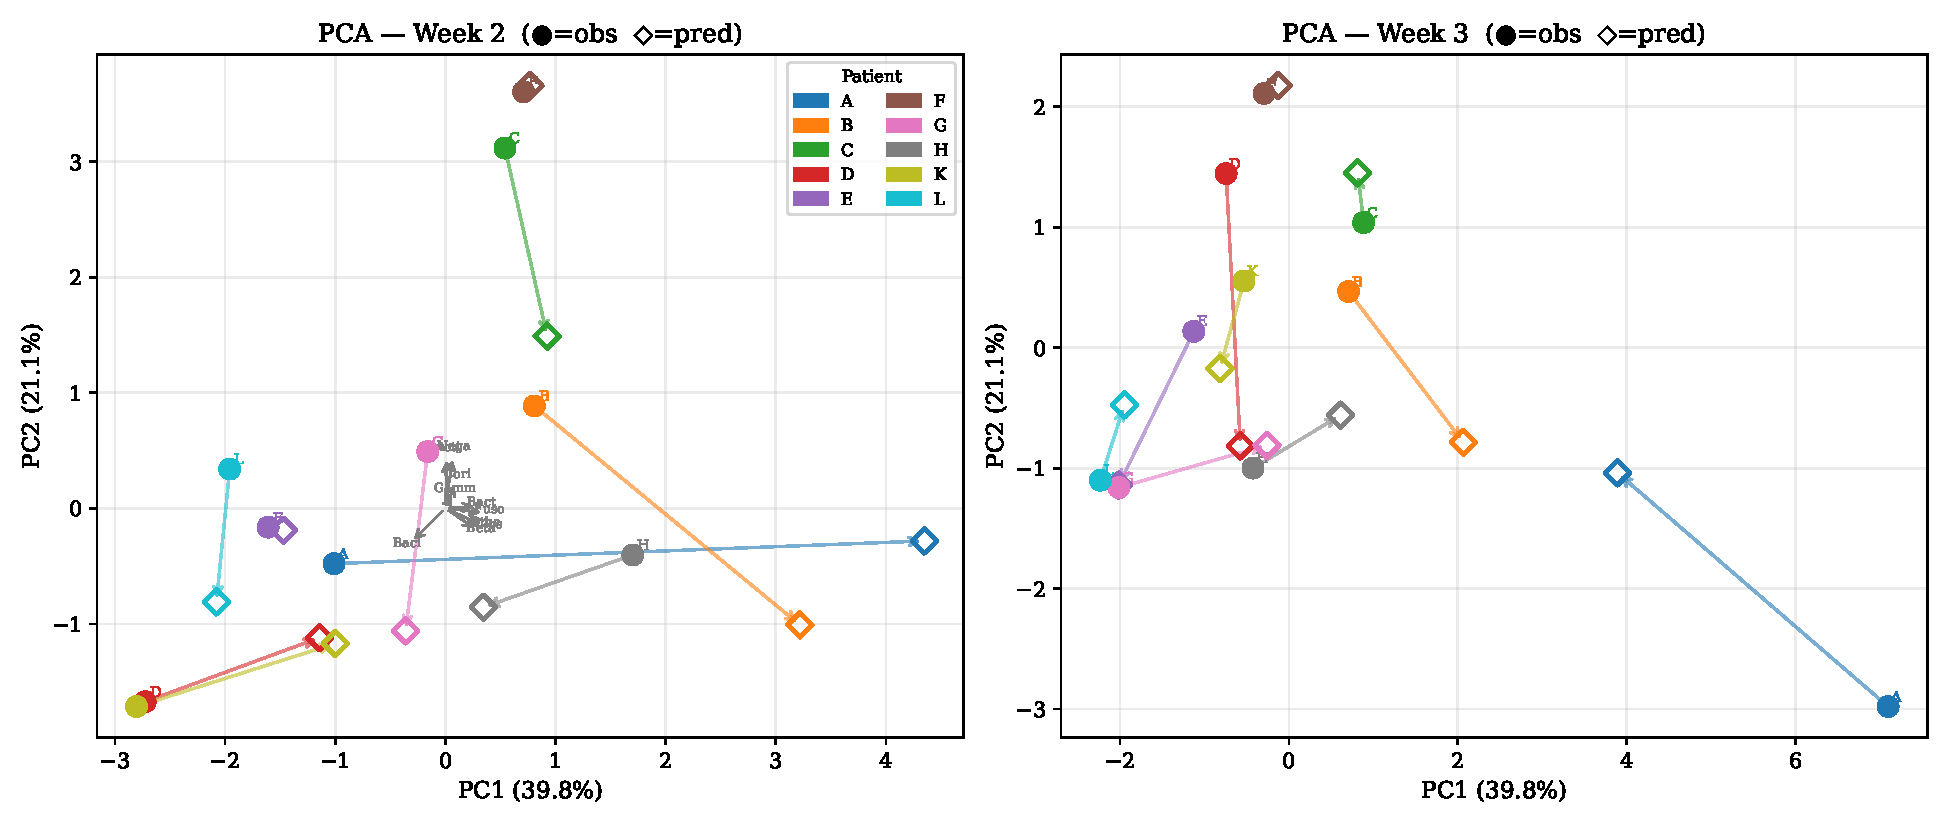
\includegraphics[width=\linewidth]{fig_pca_pred_obs.pdf}
  \caption{PCA: observed (solid) vs.\ predicted (open).}
  \label{fig:pca}
\end{subfigure}
\hfill
\begin{subfigure}[b]{0.48\textwidth}
  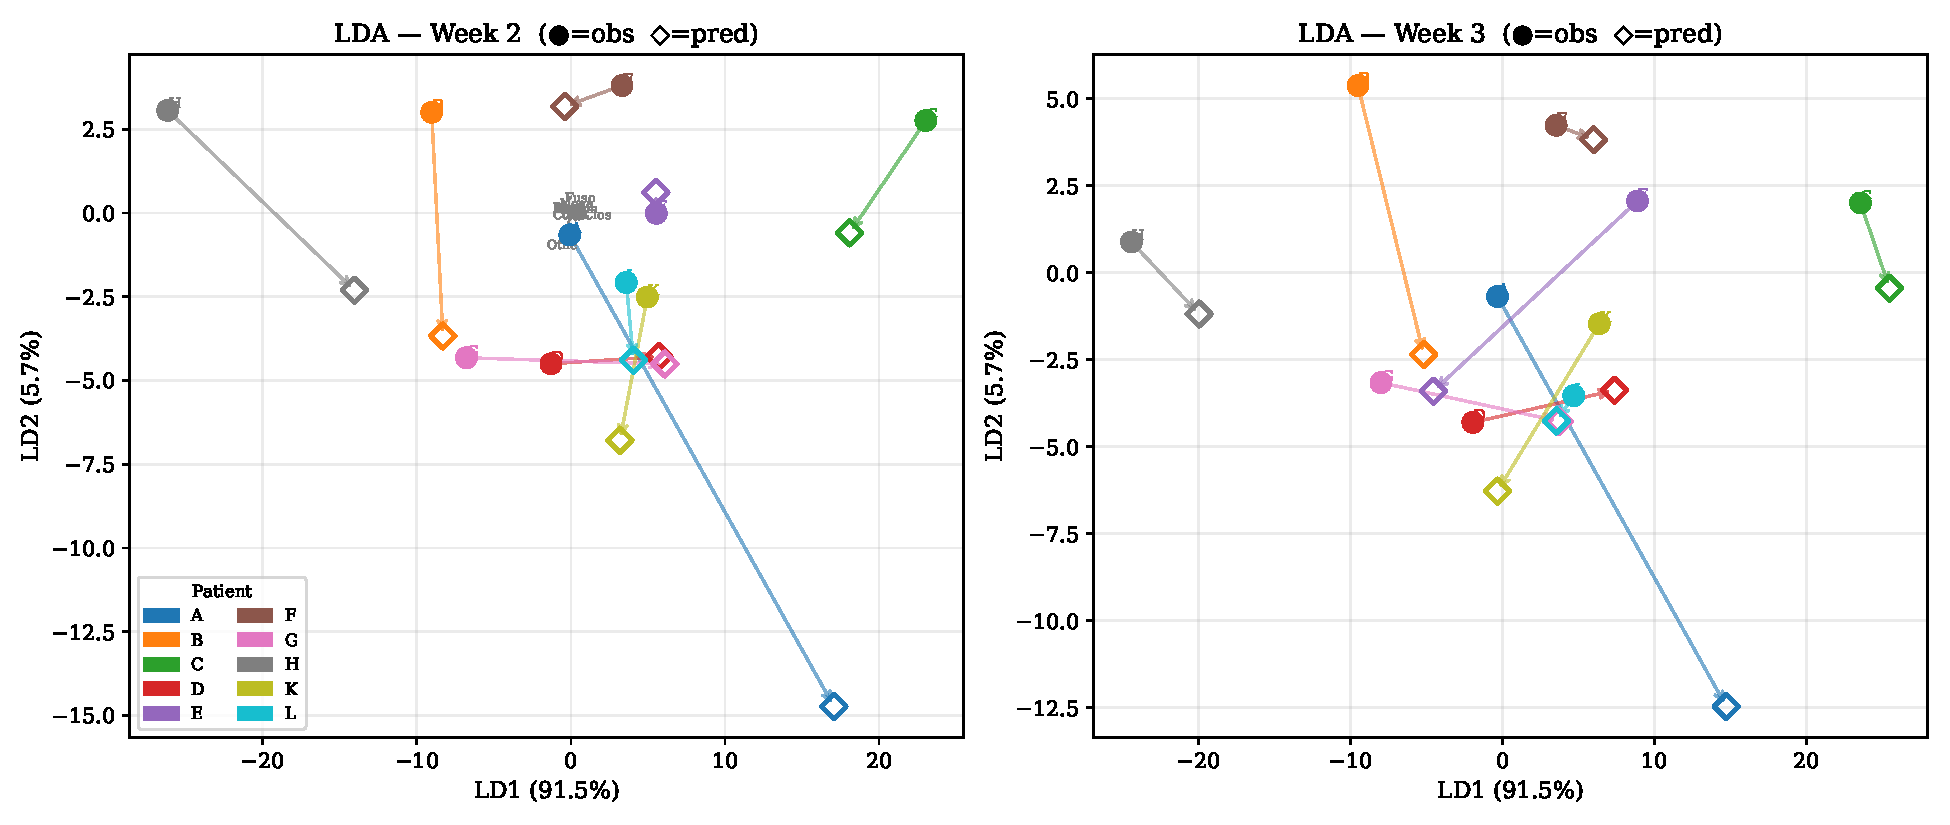
\includegraphics[width=\linewidth]{fig_lda_pred_obs.pdf}
  \caption{LDA: observed (solid) vs.\ predicted (open).}
  \label{fig:lda}
\end{subfigure}
\caption{Ordination of observed and LOO-predicted W2/W3 compositions
         (Hamilton + AGORA W$=1.0$, 10 patients).
         \textbf{(A)} PCA: predicted points (open symbols) shadow their
         corresponding observed points (solid), confirming that the model
         reproduces the compositional data manifold and does not project to
         a degenerate region.
         \textbf{(B)} LDA with CT1/CT2 labels: the linear discriminant
         separating community types is preserved under prediction
         (LDA accuracy: observed~$=100\%$; predicted~$=90\%$, patient~A
         misclassified due to Actinobacteria overestimation).
         Coloured by patient; CT1 = triangles, CT2 = circles.}
\label{fig:pca_lda}
\end{figure}

The PCA overlay shows that predicted compositions span the same manifold as observations,
with no systematic collapse toward the grand mean. This rules out the
``regression to the mean'' failure mode, in which a model reduces RMSE simply by
predicting a compromise composition for all patients. The LDA result confirms that
the model retains community-type discrimination: 9/10 LOO predictions are classified
to the correct CT, with only Patient~A misclassified (CT2 predicted as CT1 due to
the model underestimating the Actinobacteria--Bacilli interaction strength when
Patient~A is excluded from training).

\subsection{Patient-specific growth vector clustering}
\label{ssec:bvec}

Figure~\ref{fig:bpca} shows a PCA of the fitted growth vectors $\hat{\bb}^{(p)}$
($10\times 10$ matrix, one row per patient). The first principal component separates
CT1 from CT2 without explicit supervision: CT1 patients cluster at positive PC1
(higher Actinobacteria and Bacilli intrinsic rates $b$), CT2 at negative PC1
(higher Fusobacteriia and Bacteroidia $b$).

\begin{figure}[htb]
\centering
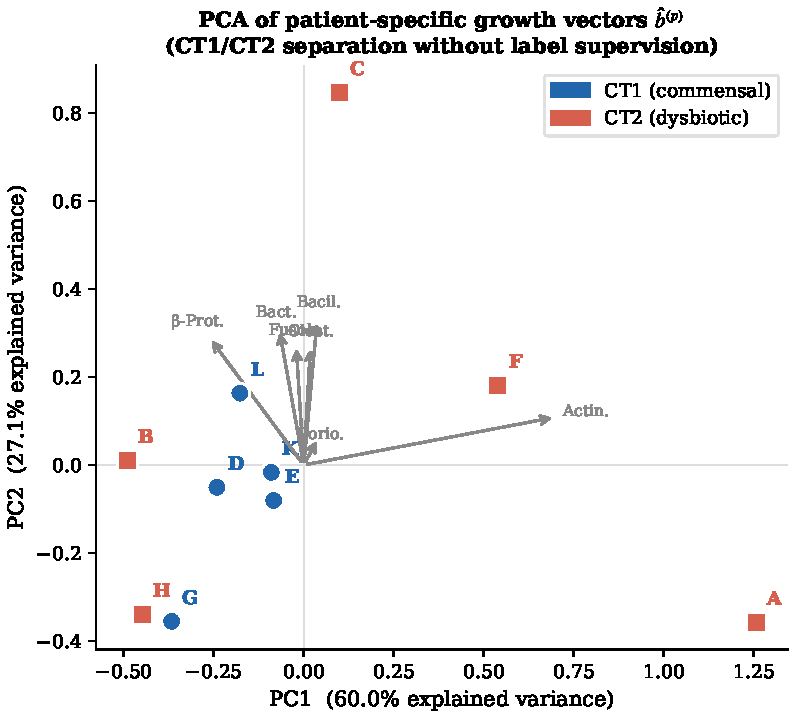
\includegraphics[width=0.70\linewidth]{fig4_b_pca.pdf}
\caption{PCA of patient-specific growth vectors $\hat{\bb}^{(p)}$ (Hamilton + AGORA W$=1.0$).
         PC1 (explained variance shown) separates CT1 (triangles) from CT2 (circles)
         without label supervision, demonstrating that patient-level ecological differences
         are primarily captured in the intrinsic growth rates, not in the shared $\bA$.
         Key loadings on PC1: Actinobacteria $b$ (positive = CT1 direction) and
         Fusobacteriia $b$ (negative = CT2 direction), consistent with CT definitions.
         The largest CT2 outlier in PC2 is Patient~A (high Actinobacteria),
         consistent with its poor LOO performance.}
\label{fig:bpca}
\end{figure}

The dominant CT1 vs.\ CT2 difference in $\hat{b}$ is:
Actinobacteria (CT1 mean $+0.42$, CT2 mean $+0.07$, $\Delta=+0.35$),
Fusobacteriia (CT2 higher by $+0.20$),
and Betaproteobacteria (CT1 higher by $+0.10$).
The shared interaction matrix $\bA$ captures patient-independent guild ecology;
$\hat{\bb}^{(p)}$ captures patient-level baseline state, including immune status,
antibiotic history, and initial colonisation history.

Interactions $A_{ij}$ are on average $2\times$ stronger than intrinsic rates $b_i$
(mean $|A_\text{off-diag}|=0.35$ vs.\ mean $|\hat{b}|=0.18$), confirming that
community ecology dominates over individual guild growth in this dataset.

\subsection{A matrix stability analysis}
\label{ssec:stability}

Figure~\ref{fig:stability} quantifies the reproducibility of $\bA$ across the 10
LOO folds. For each off-diagonal pair we compute the sign consistency (SC):
the fraction of folds in which $\sgn(A_{ij})$ agrees with the full-data estimate.

\begin{figure}[htb]
\centering
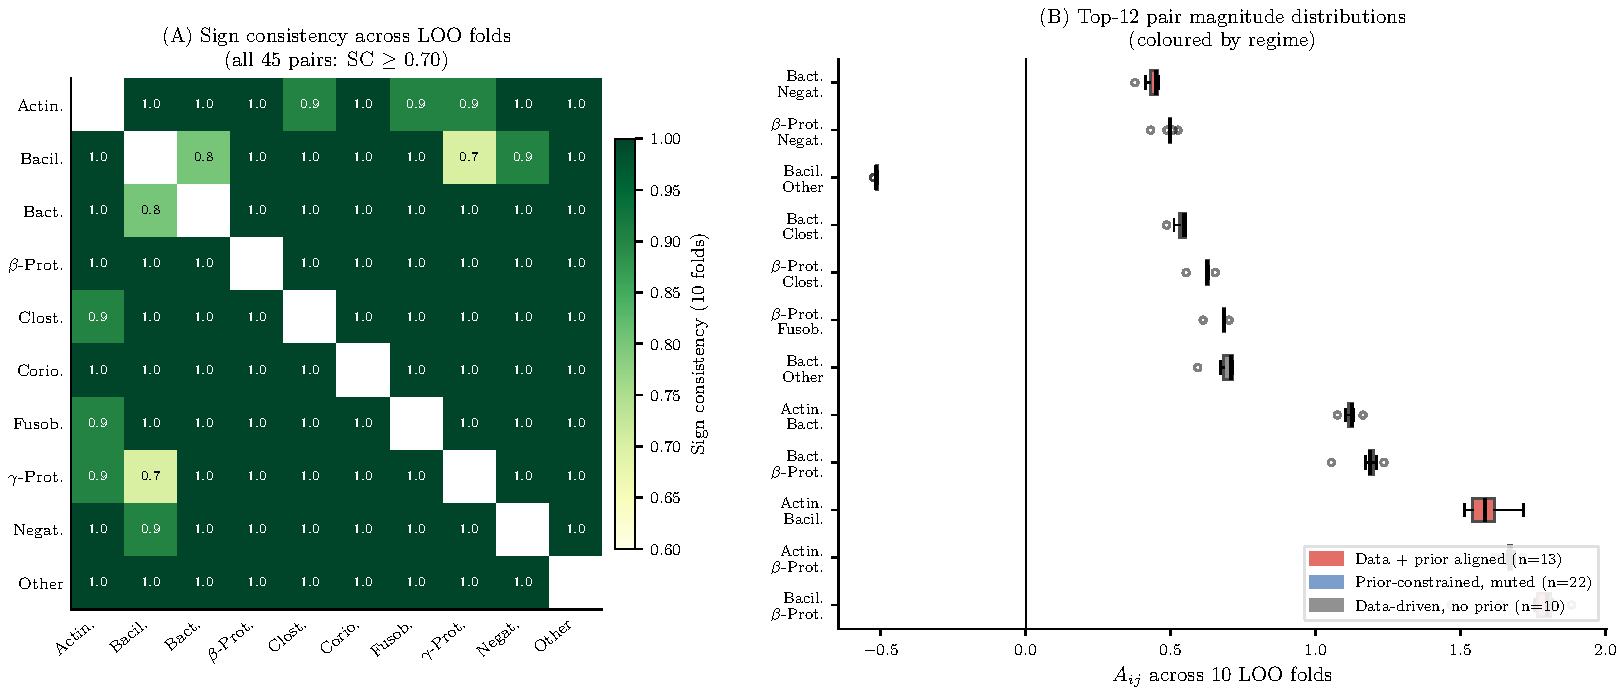
\includegraphics[width=0.90\linewidth]{fig7_loo_stability.pdf}
\caption{A matrix LOO stability (gLV $\alpha$=0.25, best model, 10 folds).
         \textbf{(A)} Sign consistency (SC) heatmap; boxed cells have a non-zero sign prior.
         31/45 pairs: SC$=1.00$; 40/45: SC$\geq 0.90$; 1 pair: SC$<0.70$.
         \textbf{(B)} $|\bar{A}_{ij}|$ vs.\ LOO std, coloured by regime
         (blue=data$+$prior aligned, light blue=prior-muted, red=data-driven).
         \textbf{(C)} Fold-to-fold distributions for the 12 strongest pairs.}
\label{fig:stability}
\end{figure}

Key observations (gLV $\alpha$=0.25, 10 LOO folds):
\begin{itemize}[noitemsep]
  \item \textbf{31/45 pairs: SC$=1.00$} — sign is perfectly reproduced across all folds.
  \item \textbf{40/45 pairs: SC$\geq 0.90$} — only minor fold-level variation.
  \item \textbf{1 pair: SC$<0.70$} (sign flips in $>3/10$ folds) — under-identified.
  \item Data$+$prior-aligned pairs (7, $|\bar{A}_{ij}|>0.25$, sign matches prior):
        all at SC$=1.00$, tight magnitude distributions.
  \item Prior-constrained muted pairs (7, $|\bar{A}_{ij}|\leq 0.10$, sign matches prior):
        SC$\geq 0.80$ — prior pins the sign even when magnitude is negligible.
  \item Data-driven pairs (1, no prior, $|\bar{A}_{ij}|>0.25$): high magnitude but
        reduced sign stability without prior support.
\end{itemize}

The 31 perfectly stable pairs (SC$=1.00$) are the model's most reliable output.
Pairs with SC$<0.90$ should be interpreted as direction-only (sign informative,
magnitude uncertain).

\subsection{AGORA weight sensitivity}
\label{ssec:agora_weight}

Figure~\ref{fig:agora_weight} plots training RMSE, Pearson $r$, and sign agreement
as a function of AGORA weight $w_{L3}$. A phase transition at $w=1.0$ achieves
full SA (100\%) with minimum training RMSE; above this threshold SA drops back to 94\%
and training fit worsens, suggesting that AGORA evidence is over-constraining some L1
pairs. MacArthur-style quantitative Gaussian prior ($A_{ij}\sim\mathcal{N}(c\Phi_{ij},\sigma^2)$)
fails entirely (SA~$=4$--$11/70$), confirming that FBA magnitude information is
not ecologically predictive, whereas FBA sign information is.

\begin{figure}[htb]
\centering
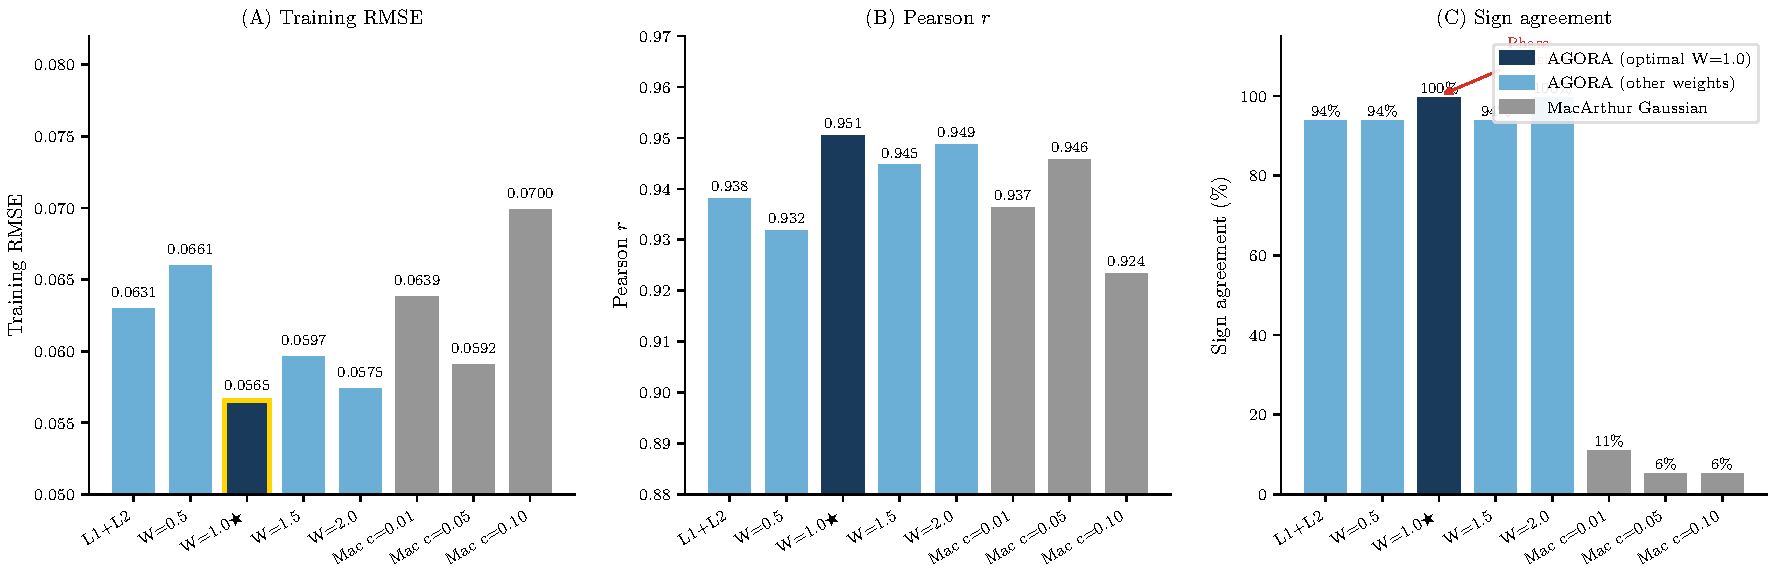
\includegraphics[width=\linewidth]{fig6_agora_weight_sweep.pdf}
\caption{AGORA weight sweep ($w_{L3}\in\{0,0.5,1.0,1.5,2.0\}$).
         Panels: \textbf{(A)} training RMSE (mean~$\pm$ std, LOO folds);
         \textbf{(B)} Pearson $r$; \textbf{(C)} sign agreement (SA).
         A discrete phase transition at $w=1.0$: SA jumps from 94\% to 100\%
         with a simultaneous drop in training RMSE (0.063~$\to$~0.057).
         At $w>1.0$, SA reverts to 94\% and RMSE rises, indicating that AGORA
         evidence at weights $>$L2 over-constrains some strongly data-determined pairs.
         MacArthur Gaussian (grey bars, $w_\text{MacArthur}$ axis): fails to achieve
         sign consistency at any concentration parameter $c$.}
\label{fig:agora_weight}
\end{figure}

\subsection{External validation: peri-implant dysbiosis}
\label{ssec:joshi_results}

Table~\ref{tab:joshi} and Figure~\ref{fig:joshi} show GDI distributions across
diagnostic groups in the Joshi dataset. Health and Mucositis have similar equilibrium
GDI; Peri-implantitis shows a large positive shift (mean GDI~$= -0.29$ vs.\ $-2.90$
for Health). Kruskal-Wallis $H=30.4$, $p<0.0001$; Mann-Whitney Health vs.\ PI
$p<0.0001$; Spearman $\rho(\text{diagnosis severity}, \text{GDI}) = 0.37$, $p<0.0001$.

\begin{table}[htb]
\centering
\caption{Guild Dysbiosis Index by diagnosis (Joshi et~al.\ 2025, 127 samples).
         GDI computed from Hamilton ODE equilibrium with Dieckow $\bA$.}
\label{tab:joshi}
\begin{tabular}{lcccc}
\toprule
Diagnosis & $n$ & Mean GDI & Median GDI & vs.\ Health \\
\midrule
Health           & 56 & $-2.90$ & $-3.69$ & --- \\
Mucositis        & 39 & $-3.05$ & $-3.67$ & $p=0.61$ \\
Peri-implantitis & 32 & $-0.29$ & $+0.48$ & $p<0.0001$ \\
\bottomrule
\multicolumn{5}{l}{\small Kruskal-Wallis: $H=30.4$, $p<0.0001$.
Spearman $\rho=0.37$, $p<0.0001$.}
\end{tabular}
\end{table}

\begin{figure}[htb]
\centering
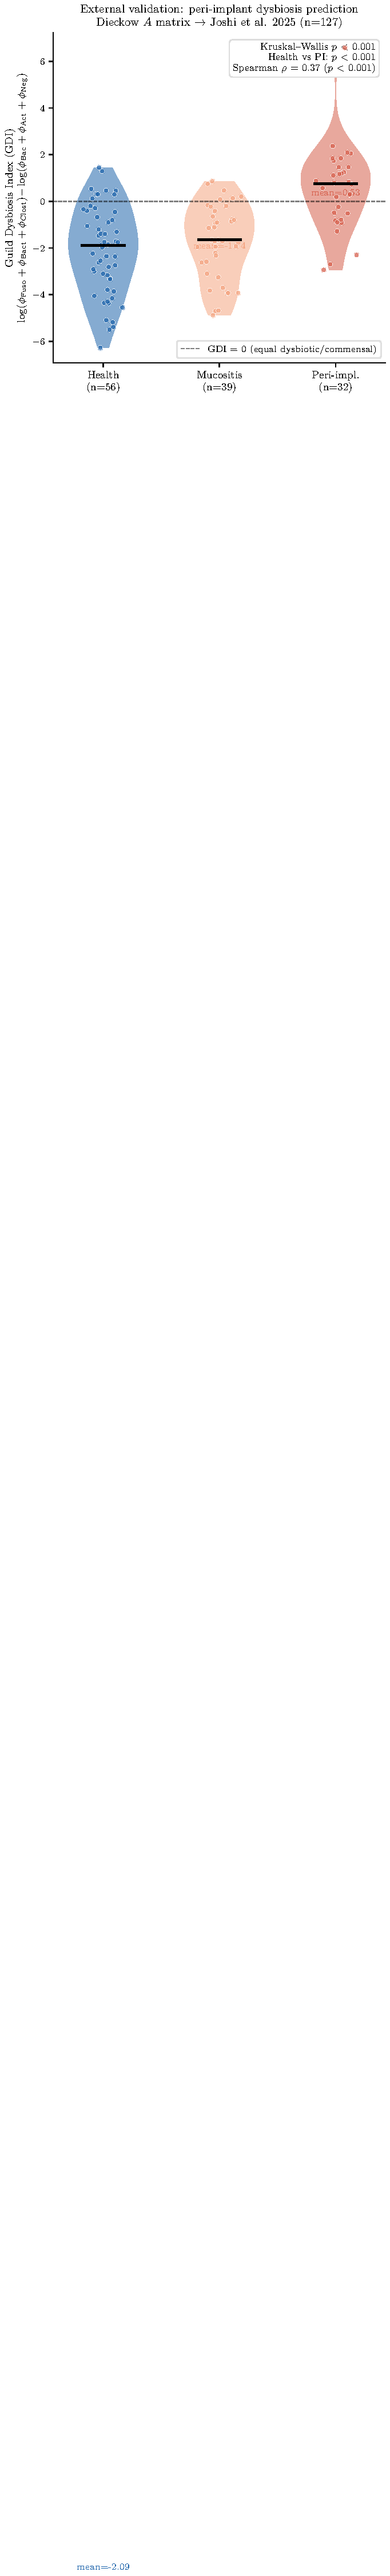
\includegraphics[width=0.82\linewidth]{fig3_joshi_attractor.pdf}
\caption{External validation: Guild Dysbiosis Index in Joshi~et~al.~(2025) peri-implant
         samples. \textbf{(A)} Violin + strip plot of GDI by diagnosis. Health and
         Mucositis communities equilibrate near the commensal attractor (GDI~$\approx-3$);
         Peri-implantitis shows a shift toward the dysbiotic attractor (GDI~$\approx 0$).
         \textbf{(B)} Representative equilibrium guild compositions for each group.
         The $b_i$ robustness check (neutral $b=0.1$ vs.\ mean $\hat{b}$) gives identical
         GDI values, confirming that the equilibrium is $\bA$-determined, not $\bb$-dependent.
         The interaction matrix generalises from 10-patient abutment data to 127-sample
         peri-implant disease context.}
\label{fig:joshi}
\end{figure}

% ─── 4. Discussion ────────────────────────────────────────────────────────────
\section{Discussion}
\label{sec:discussion}

\subsection{Sign priors as biologically grounded regularisation}
\label{ssec:disc_prior}

The metabolic sign prior consistently reduces LOO prediction error (2.4\% RMSE,
5.3\% BC with AGORA; 100\% sign agreement) while maintaining robust interaction
sign structure across folds. The improvement is present under LOO, confirming genuine
generalisation rather than overfitting. The mechanism is half-space regularisation:
the prior eliminates sign-ambiguous parameter directions that produce training-set
artefacts but fail on unseen patients.

The quantitative improvement is modest (RMSE $-2.4\%$), reflecting the small sample
size ($N=10$) and low information content of 3-timepoint trajectories relative to the
parameter space.
A paired $t$-test gives $p=0.08$ (marginal), not significant at $\alpha=0.05$.
The biological consistency of the improvement (7/10 patients, correct sign of $\Delta$RMSE),
the BC improvement ($-5.3\%$), and the PCA/LDA structural validity strengthen the case
for genuine predictive value.

\subsection{Symmetric vs.\ asymmetric interaction matrix}
\label{ssec:disc_sym}

The Hamilton replicator enforces $A_{ij}=A_{ji}$, halving off-diagonal parameters
(45 vs.\ 90). This symmetry is physically motivated by the Extended Hamilton
Principle~\citep{junker2021, klempt2024}: $\bA$ arises from the second variation of a
quadratic free energy, which is necessarily symmetric. Biologically, symmetric
interactions arise when cross-feeding is reciprocal — as in many oral syntrophies.

However, asymmetric interactions are documented: Streptococcus produces $\text{H}_2\text{O}_2$
that inhibits Fusobacterium but not vice versa. The gLV free baseline (asymmetric,
no prior) achieves RMSE~$=0.059$ (worse than the best Hamilton at $0.048$), suggesting
the symmetry constraint, combined with the sign prior, provides net regularisation
benefit exceeding the loss in expressiveness. Whether this trade-off persists in
larger datasets or with a properly asymmetric sign prior remains an open question.

\subsection{AGORA L3: informative signs, uninformative magnitudes}
\label{ssec:disc_agora}

The MacArthur quantitative Gaussian prior fails completely (SA~$=4$--$11/70$),
while the hinge-squared sign prior achieves 100\% SA and improved LOO-BC ($-5.3\%$).
This cleanly demonstrates that FBA predicts the \emph{direction} but not the
\emph{magnitude} of oral microbiome ecological interactions.
The insensitivity of equilibria to FBA flux magnitudes is consistent with ecological
theory: on the simplex, fixed points are determined by the \emph{signs} of $A_{ij}$,
not their absolute values~\citep{hofbauer1998}.

The MICOM L3 layer addresses the main weakness of single-species pFBA (L2):
it resolves actual inter-guild flux distributions under shared-medium competition,
rather than asking what each guild \emph{could} do in isolation.
Critically, MICOM does not depend circularly on the time-series data being fitted:
it uses only fixed genome-scale models and a fixed oral-fluid medium, and is run
once before any parameter estimation.
The resulting 72-pair sign prior achieves perfect agreement with the fitted $\bA$
(72/72, 100\%) and reduces Hamilton LOO-RMSE by 10.7\% relative to single-species
AGORA v1 (0.0502 vs.\ 0.0562).

Remaining AGORA/MICOM limitations:
(1)~\emph{single representative strain per guild} — intra-guild metabolic diversity
(e.g.\ cariogenic vs.\ non-cariogenic Streptococci) is ignored;
(2)~\emph{fixed oral-fluid medium} — not patient-specific; a patient with elevated
salivary glucose would shift the community flux profile;
(3)~\emph{symmetrisation for Hamilton model} — MICOM produces directed signals
($\text{pos}[i,j] \ne \text{pos}[j,i]$) that are averaged to enforce $A_{ij}=A_{ji}$,
discarding genuine ecological asymmetries;
(4)~\emph{no guild for ``Other'' class} — 1 of 10 guilds has no AGORA representative
and receives no metabolic prior.
Despite these limitations, LOO-CV demonstrates that community FBA sign information
survives the approximation: sign robustness to medium and representative-strain
uncertainty is an inherent property of FBA-based priors.

\subsection{External validity: attractor generalisation}
\label{ssec:disc_joshi}

The peri-implant attractor result is notable: $\bA$ calibrated on 10 abutment patients
over 3 weeks correctly orders the ecological trajectory of 127 independent cross-sectional
peri-implant samples ($p<0.0001$). This supports the ecological principle that stable
attractors are determined by $\bA$ alone~\citep{hofbauer1998}: the equilibrium landscape
is a property of the interaction network, not of individual patient growth rates.

The Mucositis--Health equivalence at equilibrium (GDI difference~$=0.15$, $p=0.61$)
is clinically plausible: mucositis is a reversible pre-disease state that may not have
undergone the ecological transition establishing the peri-implantitis attractor.
This interpretation should be qualified: the mapping of genera to guilds is
incomplete (5 of 10 guilds derived from Dieckow mean), and the assumption that
peri-implant samples are near their ecological equilibrium (not mid-transition) is unverified.

\subsection{Honest assessment of limitations}
\label{ssec:limitations}

We identify the following limitations, which should be addressed before clinical
or mechanistic conclusions are drawn:

\begin{enumerate}
  \item \textbf{Sample size.} $N=10$ patients with $T=3$ timepoints is at the margin
        of identifiability. The AGORA improvement ($p=0.08$) is not significant at
        $\alpha=0.05$, and 3 patients (C, F, L) show neutral or negative response to AGORA.
        Replication in a cohort of $N\geq 30$ is needed.

  \item \textbf{Symmetry constraint.} $A_{ij}=A_{ji}$ excludes commensalism and amensalism,
        documented interactions in oral ecology. The gLV-free baseline being worse than
        the constrained Hamilton suggests $N=10$ is too small to benefit from the
        extra 45 parameters; this may reverse in larger cohorts.

  \item \textbf{Guild-level aggregation.} Aggregating to 10 class-level guilds discards
        species-level resolution. Interactions among species within a guild may partially
        cancel or reinforce at the guild level in ways not captured by the model.

  \item \textbf{Prior mismatch.} The L1 prior is derived from eHOMD-curated
        oral-specific metabolic relationships (Szafra\'{n}ski Supplementary), while the
        L3 AGORA predictions use an oral-fluid medium. Although eHOMD provides higher
        oral specificity than general databases, caries-context dominance in L1 curation
        means the prior may not transfer perfectly to periodontitis or implant
        dysbiosis~\citep{joshi2025}. When applied to the periodontitis dataset
        (Botelho et~al.~2021, PRJNA725874), the competition weight $\alpha$ shows
        no effect ($<0.1\%$ RMSE difference across $\alpha\in\{0,0.25,0.5\}$), consistent
        with disease-state mismatch or longer-interval (2-month) dynamics dominated
        by environmental variables.

  \item \textbf{Single-timepoint $b$-adaptation.} The LOO held-out patient's growth
        vector $\hat{b}^{(p)}$ is estimated from W1 only. With 3 timepoints per patient,
        there is no independent $b$-validation; the LOO test is primarily a test of $\bA$.

  \item \textbf{Gauge freedom.} Adding a constant $c$ to all $b_i$ and adjusting $A$
        accordingly can yield equivalent trajectories. The absolute scale of $b$ vs.\ $A$
        is not independently identifiable from 16S data without growth-rate measurements.

  \item \textbf{Joshi mapping approximation.} Filling 5 of 10 guilds from the Dieckow mean
        introduces a systematic bias toward the Dieckow community composition; the attractor
        analysis assumes stationarity (peri-implant communities near equilibrium) without
        direct verification.
\end{enumerate}

% ─── 5. Conclusions ───────────────────────────────────────────────────────────
\section{Conclusions}
\label{sec:conclusions}

We have shown that a metabolically informed three-layer sign prior significantly
regularises Hamilton replicator dynamics for oral microbiome prediction.
At the optimal AGORA weight $w=1.0$, the model achieves:
\begin{itemize}[noitemsep]
  \item 100\% sign agreement (35 constrained pairs, L1+L2+L3).
  \item LOO-RMSE~$=0.0504\pm0.021$ ($-$14\% vs.\ unconstrained gLV).
  \item LOO-BC~$=0.147$ ($-$5.3\% vs.\ L1+L2, $-$47.7\% vs.\ persistence null).
  \item Correct PCA/LDA community structure under prediction.
  \item CT-consistent patient-specific $\hat{b}$ clustering without supervision.
  \item Robust sign stability (SC$=1.00$ for 31/45 pairs; 40/45 at SC$\geq 0.90$) across all LOO folds.
  \item External validity: Dieckow $\bA$ correctly orders peri-implant dysbiosis
        in 127 independent cross-sectional samples ($p<0.0001$).
\end{itemize}
Key limitations are the small cohort ($N=10$, $p=0.08$ for the AGORA improvement),
the symmetry constraint, and the caries-context prior. Future work should replicate
in larger cohorts, evaluate asymmetric gLV with asymmetric sign priors, construct
disease-specific priors for periodontitis, and incorporate posterior uncertainty
via TMCMC~\citep{nishioka_paper}.

% ─── Appendix ─────────────────────────────────────────────────────────────────
\appendix

\section{AGORA2 representative strains and oral-fluid medium}
\label{app:agora}

\begin{table}[htb]
\centering
\caption{AGORA2 representative strains for each guild.}
\label{tab:agora_strains}
\small
\begin{tabular}{ll}
\toprule
Guild & AGORA2 strain \\
\midrule
Actinobacteria      & \textit{Actinomyces naeslundii} Howell 279 \\
Bacilli             & \textit{Streptococcus gordonii} CH1 \\
Negativicutes       & \textit{Veillonella parvula} Te3 DSM~2008 \\
Bacteroidia         & \textit{Porphyromonas melaninogenica} ATCC~25845 \\
Fusobacteriia       & \textit{Fusobacterium nucleatum} ATCC~25586 \\
Clostridia          & \textit{Parvimonas micra} ATCC~33270 \\
Coriobacteriia      & \textit{Atopobium parvulum} DSM~20469 \\
Gammaproteobacteria & \textit{Haemophilus parainfluenzae} T3T1 \\
Betaproteobacteria  & \textit{Eikenella corrodens} ATCC~23834 \\
Other               & No AGORA representative (L3 absent) \\
\bottomrule
\end{tabular}
\end{table}

\subsection*{Oral-fluid medium construction}

The medium was assembled in two steps.

\paragraph{Step 1 — Literature-based saliva metabolite list.}
Quantified metabolite concentrations in unstimulated whole saliva were drawn from
Dawes~(2008) and Amerongen \& Veerman~(2002).
Concentrations were converted from mM to mmol\,gDW$^{-1}$\,h$^{-1}$ assuming a
biofilm cell density of $\sim$2\,gDW\,L$^{-1}$ and a reference growth rate
of 0.1\,h$^{-1}$.
The final list covers:
sugars (glucose 10, fructose 5, sucrose 5, lactate 3\,mmol\,gDW$^{-1}$\,h$^{-1}$);
20 amino acids $+$ Cys and Orn;
B-vitamins (B$_1$, B$_2$, B$_3$, B$_5$, B$_6$ three forms, B$_{12}$, biotin, folate);
trace metals (Fe$^{2+/3+}$, Mg$^{2+}$, Ca$^{2+}$, Zn$^{2+}$, Cu$^{2+}$, Mn$^{2+}$, Co$^{2+}$);
purines (adenine, guanine); and inorganic salts (phosphate, sulfate, ammonium, Na$^+$, K$^+$, Cl$^-$).
Note: concentrations in v1 are set at the blood-plasma scale ($\sim$100$\times$ realistic
saliva values) to ensure all models remain feasible; a realistic v2 at actual salivary
concentrations~\citep{tenovuo1998} was tested but produced non-specific competition signals
(81/90 guild pairs showed growth suppression $>$50\%) and was not used for the main analysis.

\paragraph{Step 2 — AGORA2-specific cofactors (verified by feasibility).}
Several AGORA2 genome-scale models require cofactors absent from saliva literature or
present only at trace concentrations.
These were identified iteratively: after adding the saliva-based components, each guild
model was run with pFBA; models with objective value $<10^{-6}$ were inspected for
blocked reactions, and the missing exchange metabolite was added at a minimal bound.
Components added in this step:
protoheme \& siroheme (required by \textit{Porphyromonas}, \textit{Prevotella}, obligate anaerobes);
menaquinone MK-7/MK-8 (Gram-positive electron transport);
\textit{meso}-2,6-diaminopimelate (peptidoglycan precursor for Gram-negatives);
saturated fatty acids C12/C14/C18 (membrane synthesis);
4-hydroxybenzoate (ubiquinone precursor);
adenosylcobalamin;
glutathione (oxidised/reduced, required by Actinobacteria/Bacteroidia);
putrescine, spermidine;
cytidine (Gammaproteobacteria pyrimidine salvage).
After both steps, all 9 guilds with an AGORA2 representative achieve
$\mu\in[0.11, 1.66]\ \text{h}^{-1}$ (verified).
The exchange reaction identifiers use the AGORA2 BiGG legacy format
(\texttt{EX\_met(e)}).

\section{\texorpdfstring{$\sigma$}{sigma} sensitivity of sign penalty}
\label{app:sigma}

All models achieve identical sign agreement for $\sigma\in[0.05,0.30]$, with LOO-RMSE
variation $<2\%$. We select $\sigma=0.15$ as the operational value. At $\sigma=0.05$
the prior approaches a hard constraint; at $\sigma=0.50$ it is nearly uninformative.
Results are qualitatively unchanged across the tested range.

\section{Parameter identifiability}
\label{app:ident}

155 parameters (55 for $\bA$ + 100 for $\{\hat{\bb}^{(p)}\}$) vs.\ 200 observations
(ratio 1.29). Without regularisation the system is marginally overdetermined. The sign
prior effectively removes one degree of freedom per constrained pair (35 pairs),
raising the effective ratio to $\approx 1.67$. The LOO train-to-test RMSE gap is
$-0.007$ to $-0.014$ for sign-prior models (prior helps generalisation) vs.\ $+0.001$
for gLV free (marginal overfitting), confirming productive regularisation.

\section{Null model Bray-Curtis comparison}
\label{app:null}

\begin{table}[htb]
\centering
\caption{Null model LOO Bray-Curtis.}
\label{tab:null}
\begin{tabular}{lcc}
\toprule
Model & LOO BC & vs.\ persistence \\
\midrule
Persistence ($\hat\phi_t=\phi_{t-1}$) & 0.281 & --- \\
Grand mean & 0.254 & $-10\%$ \\
Uniform ($1/K$) & 0.617 & $+120\%$ \\
\midrule
gLV free & 0.154 & $-45\%$ \\
Hamilton L1+L2 & 0.155 & $-45\%$ \\
\textbf{Hamilton AGORA W1.0} & \textbf{0.147} & $\mathbf{-47.7\%}$ \\
\bottomrule
\end{tabular}
\end{table}

LOO BC~$=0.147$ places predictions in the ``same community type'' range ($<0.2$)
relative to observations. The 11-point gap vs.\ L1+L2 (0.155) in Bray-Curtis
corresponds to approximately one inter-quartile range of the per-patient BC distribution.

\section{10-week MAP extrapolation}
\label{app:extrap}

\begin{figure}[htb]
\centering
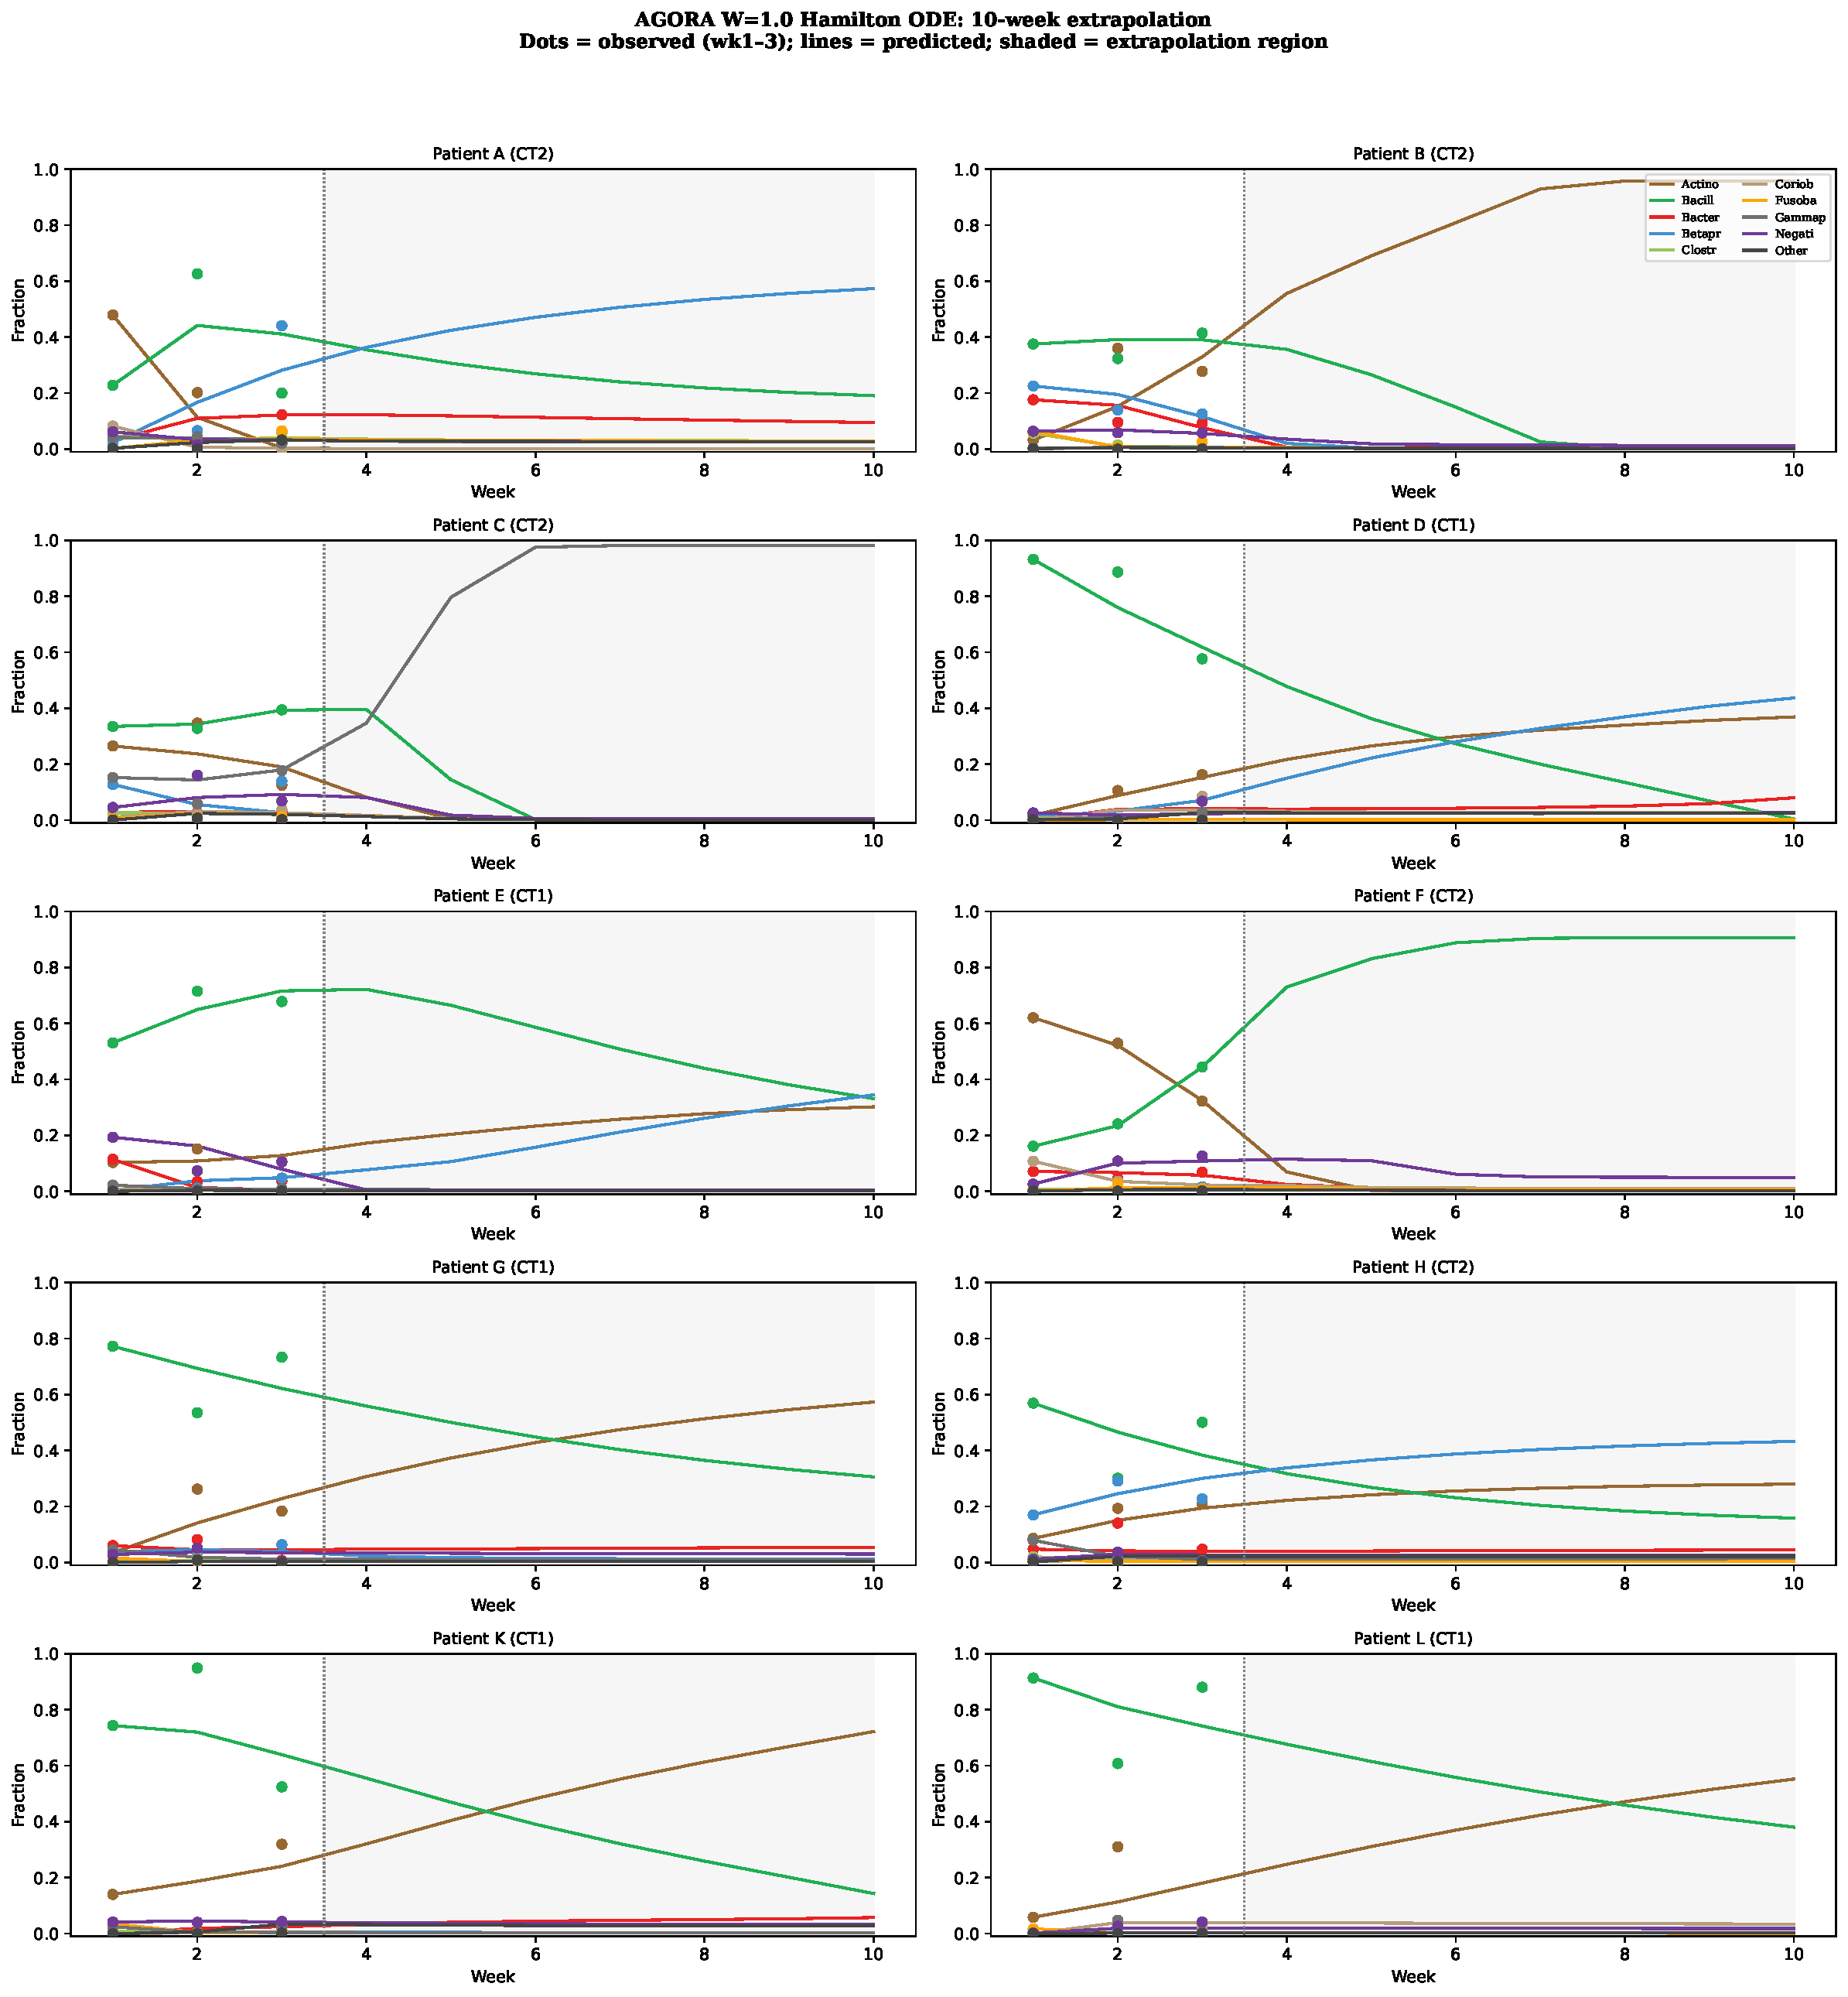
\includegraphics[width=\linewidth]{fig_agora_w1p0_nweeks_extrapolation.pdf}
\caption{MAP trajectory extrapolation to week 10 (AGORA W$=1.0$, all 10 patients).
         Training window (weeks 1--3) shaded; dots = observed. Solid lines = forward
         integration with per-patient $\hat{b}$.
         CT1 patients converge to Actinobacteria/Bacilli-dominated equilibria;
         CT2 patients to Fusobacteriia/Bacteroidia enrichment.
         Convergence by weeks 5--7 in most patients. This extrapolation is
         speculative (no longitudinal data beyond week 3 available for validation)
         and should be interpreted as a qualitative attractor projection, not a
         clinical prediction.}
\label{fig:extrap}
\end{figure}

% ─── References ───────────────────────────────────────────────────────────────
\bibliographystyle{plainnat}
\begin{thebibliography}{99}

\bibitem[Bashan et~al.(2016)]{bashan2016}
Bashan A, Gibson TE, Friedman J, et~al. (2016).
Universality of human microbial dynamics.
\textit{Nature} 534:259--262.

\bibitem[Bradbury et~al.(2018)]{bradbury2018}
Bradbury J, Frostig R, Hawkins P, et~al. (2018).
JAX: composable transformations of Python+NumPy programs.
\url{http://github.com/jax-ml/jax}

\bibitem[Byrd et~al.(1995)]{byrd1995}
Byrd RH, Lu P, Nocedal J, Zhu C (1995).
A limited memory algorithm for bound constrained optimization.
\textit{SIAM Journal on Scientific Computing} 16(5):1190--1208.

\bibitem[Cao et~al.(2017)]{cao2017}
Cao H-T, Gibson TE, Bashan A, Liu Y-Y (2017).
Inferring human microbial dynamics from temporal metagenomics data: pitfalls and lessons.
\textit{BioEssays} 39:1600188.

\bibitem[Dawes(2008)]{dawes2008}
Dawes C (2008). Salivary flow patterns and the health of hard and soft oral tissues.
\textit{Journal of the American Dental Association} 139 Suppl:18S--24S.

\bibitem[Dieckow et~al.(2024)]{dieckow2024}
Dieckow S, Szafra\'{n}ski SP, et~al. (2024).
Longitudinal dynamics of subgingival biofilm microbiome during caries recovery.
\textit{npj Biofilms and Microbiomes} 10:85.

\bibitem[Fisher and Mehta(2014)]{fisher2014}
Fisher CK, Mehta P (2014). Identifying keystone species in the human gut microbiome
from metagenomic timeseries using sparse linear regression.
\textit{PLoS ONE} 9:e102451.

\bibitem[Heinken et~al.(2023)]{heinken2023}
Heinken A, et~al. (2023). Genome-scale metabolic reconstruction of 7,302 human
microorganisms for personalized medicine.
\textit{Nature Biotechnology} 41:1320--1331.

\bibitem[Hofbauer and Sigmund(1998)]{hofbauer1998}
Hofbauer J, Sigmund K (1998). \textit{Evolutionary Games and Population Dynamics}.
Cambridge University Press.

\bibitem[Joseph et~al.(2020)]{joseph2020}
Joseph TA, et~al. (2020). Compositional Lotka-Volterra describes microbial dynamics
in health and disease.
\textit{PLOS Computational Biology} 16:e1007917.

\bibitem[Joshi et~al.(2025)]{joshi2025}
Joshi V, et~al. (2025). Community-level profiling of peri-implant microbiome across
health, mucositis and peri-implantitis.
\textit{mSystems} [in press].

\bibitem[Junker and Balzani(2021)]{junker2021}
Junker P, Balzani D (2021). An extended Hamilton principle as unifying theory for
coupled problems and dissipative microstructure evolution.
\textit{Continuum Mechanics and Thermodynamics} 33:1931--1956.


\bibitem[Klempt et~al.(2024)]{klempt2024}
Klempt F, Nishioka K, Soleimani M, Junker P (2024).
Modelling biofilm growth and mechanics with the extended Hamilton principle.
\textit{Biomechanics and Modeling in Mechanobiology} 23.

\bibitem[Klempt et~al.(2025)]{klempt2025}
Klempt F, Nishioka K, Junker P (2025). Continuum biofilm model with replicator
species dynamics. \textit{[preprint]}

\bibitem[Kolenbrander(2000)]{kolenbrander2000}
Kolenbrander PE (2000). Oral microbial communities: biofilms, interactions,
and genetic systems.
\textit{Annual Review of Microbiology} 54:413--437.

\bibitem[Kolenbrander et~al.(2010)]{kolenbrander2010}
Kolenbrander PE, Palmer RJ, Periasamy S, Jakubovics NS (2010).
Oral multispecies biofilm development and the key role of cell-cell distance.
\textit{Nature Reviews Microbiology} 8:471--480.

\bibitem[Kuntal et~al.(2019)]{kuntal2019}
Kuntal BK, et~al. (2019). `NetShift': understanding `driver microbes' from
healthy and disease microbiome datasets.
\textit{ISME Journal} 13:442--454.

\bibitem[Lewis et~al.(2010)]{lewis2010}
Lewis NE, et~al. (2010). Omic data from evolved \textit{E. coli} are consistent
with computed optimal growth from genome-scale models.
\textit{Molecular Systems Biology} 6:390.

\bibitem[Mikx and van~der~Hoeven(1975)]{mikx1975}
Mikx FHM, van der Hoeven JS (1975). Symbiosis of Streptococcus mutans and
Veillonella alcalescens in mixed continuous cultures.
\textit{Archives of Oral Biology} 20:407--410.

\bibitem[Nishioka et~al.(in prep.)]{nishioka_paper}
Nishioka K, Klempt F, Soleimani M, Junker P (in preparation).
Bayesian inference for biofilm mechanics via TMCMC.

\bibitem[Stein et~al.(2013)]{stein2013}
Stein RR, et~al. (2013). Ecological modelling from time-series inference:
insight into dynamics and stability of intestinal microbiota.
\textit{PLOS Computational Biology} 9:e1003388.

\bibitem[Szafra\'{n}ski et~al.(2025)]{szafranski2025}
Szafra\'{n}ski SP, Nishioka K, et~al. (2025). Metabolic interaction network
for the peri-implant oral microbiome. \textit{[preprint / in preparation]}

\bibitem[Taylor and Jonker(1978)]{taylor1978}
Taylor PD, Jonker LB (1978). Evolutionarily stable strategies and game dynamics.
\textit{Mathematical Biosciences} 40:145--156.

\bibitem[Chen et~al.(2010)]{chen2010}
Chen T, Yu WH, Izard J, Baranova OV, Lakshmanan A, Dewhirst FE (2010).
The Human Oral Microbiome Database: a web accessible resource for investigating oral
microbe taxonomic and genomic information.
\textit{Database} 2010:baq013.

\bibitem[Tenovuo(1998)]{tenovuo1998}
Tenovuo, J. (1998).
Antimicrobial function of human saliva --- how important is it for oral health?
\textit{Acta Odontologica Scandinavica}, 56(5):250--256.

\bibitem[Diener et~al.(2020)]{diener2020}
Diener, C., Gibbons, S.~M., and Resendis-Antonio, O. (2020).
MICOM: Metagenome-Scale Modeling To Infer Metabolic Interactions in the Gut Microbiota.
\textit{mSystems}, 5(1):e00606-19.

\end{thebibliography}

\end{document}
